% !TEX program = xelatex
% Cards format — auto-generated from keymaps.tex by cards-convert.mjs
\documentclass[11pt]{article}

\usepackage{fontspec}
\usepackage{unicode-math}
\usepackage{xeCJK}
% Hiragino Sans is macOS-native and renders proper Japanese kanji forms
% (the papermill default Droid Sans Japanese is absent here and falls back to
% Chinese-variant glyphs). Hand-deployed build; if the oven is ever re-enabled,
% swap to a Linux JP font (e.g. Noto Sans CJK JP).
\setCJKmainfont{Hiragino Sans}
% Latin Modern by OTF filename (not font name): xelatex on macOS (Core
% Text, no fontconfig) cannot resolve "Latin Modern Roman" by name, which
% silently produced ~4KB broken card PDFs. kpathsea finds the OTFs in
% texmf-dist on both macOS and the oven's Linux xelatex.
\setmainfont{lmroman10-regular.otf}[
  BoldFont=lmroman10-bold.otf,
  ItalicFont=lmroman10-italic.otf,
  BoldItalicFont=lmroman10-bolditalic.otf,
]
\setsansfont{lmsans10-regular.otf}[
  BoldFont=lmsans10-bold.otf,
  ItalicFont=lmsans10-oblique.otf,
  BoldItalicFont=lmsans10-boldoblique.otf,
]
\setmonofont{lmmono10-regular.otf}[Scale=0.88,
  BoldFont=lmmonolt10-bold.otf,
  ItalicFont=lmmono10-italic.otf,
]


\usepackage{graphicx}
\graphicspath{{./}{figures/}}
\usepackage{booktabs}
\usepackage{tabularx}
\usepackage{adjustbox}
\usepackage{ragged2e}
\usepackage{microtype}
\usepackage{natbib}



\makeatletter
\def\input@path{{../}}
\makeatother
\usepackage{ac-paper-cards}

% Extra commands from base paper
\newcommand{\dmn}[2]{\textcolor{#1}{\textbf{#2}}}
\newcommand{\qrc}[1]{\raisebox{\dimexpr-0.5\height+0.8ex\relax}{\includegraphics[height=0.74cm]{figures/qr/#1.png}}}
\newcommand{\klang}[2]{\href{https://papers.aesthetic.computer/keymaps-social-software-26-arxiv-cards#2.pdf}{\color{acgray}#1}}
\newcommand{\klanghere}[1]{{\bfseries\color{acpink}#1}}
\newcommand{\klangsep}{{\color{acgray!60}\,\textperiodcentered\,}}
\definecolor{keyfill}{RGB}{248,248,250}
\definecolor{keystroke}{RGB}{160,156,170}
\definecolor{keymapped}{RGB}{180,72,135}
\definecolor{keysharp}{RGB}{52,52,64}
\definecolor{acblue}{RGB}{42,100,212}
\definecolor{acgreen}{RGB}{42,154,58}
\definecolor{acorange}{RGB}{216,120,0}

% Carried from keymaps.tex: macros/packages cards-convert does not extract
% (\key/\keys live inside \makeatletter; the version stamp + colored-table
% and figure-caption commands come from the grown source paper).
\usepackage{tikz}
\usetikzlibrary{calc,positioning,shapes.geometric,arrows.meta}
\usepackage{caption}
\usepackage{colortbl}
% \ac/\acdot already come from ac-paper-cards. Carry the keycap/hex tikz
% styles the figures use (cards-convert does not extract \tikzset).
\tikzset{
 kcap/.style={draw=keystroke, fill=keyfill, rounded corners=0.6pt,
        minimum width=0.34cm, minimum height=0.34cm,
        inner sep=0pt, font=\scriptsize\sffamily},
 kcap mapped/.style={kcap, fill=keymapped!18, draw=keymapped!60,
            text=keymapped!90},
 kcap sharp/.style={kcap, fill=keysharp, draw=keysharp,
           text=white, font=\scriptsize\sffamily\bfseries},
 hexkey/.style={regular polygon, regular polygon sides=6,
         draw=keystroke, fill=keyfill, rounded corners=0pt,
         minimum size=0.55cm, inner sep=0pt,
         font=\tiny\sffamily},
 hexkey mapped/.style={hexkey, fill=keymapped!22, draw=keymapped!70,
             text=keymapped!90},
}
\DeclareRobustCommand{\key}[1]{\tikz[baseline=(k.base)]{%
 \node[fill=keystroke, rounded corners=1.3pt, inner xsep=2.4pt,
    inner ysep=1.9pt, anchor=base, yshift=-1.2pt] at (0,0)
  {\footnotesize\ttfamily\bfseries\vphantom{A}\phantom{#1}};
 \node[draw=keystroke, line width=0.4pt, fill=keyfill,
    rounded corners=1.3pt, inner xsep=2.4pt, inner ysep=1.9pt,
    anchor=base] (k) at (0,0)
  {\footnotesize\ttfamily\bfseries\vphantom{A}#1};}}
\makeatletter
\DeclareRobustCommand{\keys}[1]{{\def\sep{}\@for\kk:=#1\do{\sep\key{\kk}\def\sep{\,}}}}
\makeatother
\InputIfFileExists{version}{}{%
 \providecommand{\paperhash}{dev}\providecommand{\paperrev}{?}}
\InputIfFileExists{history}{}{\providecommand{\paperhistory}{}}

\hypersetup{
  pdftitle={社会的ソフトウェアとしてのキーマップ：社会的契約による版管理された仮想的対象},
}

\renewcommand{\acpdfbase}{keymaps-social-software-26-arxiv}
\begin{document}

% ============================================================
% TITLE CARD
% ============================================================
\thispagestyle{empty}
\vspace*{\fill}
\begin{center}
\href{https://papers.aesthetic.computer}{
\includegraphics[height=9em]{pals}}\par\vspace{0.1em}
{\fontsize{18pt}{22pt}\selectfont\bfseries\color{acdark} 社会的ソフトウェアとしてのキーマップ}\par
\vspace{0.1em}
\vspace{0.3em}
{\normalsize\color{cyan!70!blue}\href{https://prompt.ac/@jeffrey}{\textbf{@jeffrey}}}\par
{\small\color{acgray} Aesthetic.Computer}\par
{\small\color{acgray} ORCID: \href{https://orcid.org/0009-0007-4460-4913}{0009-0007-4460-4913}}\par
\vspace{0.4em}
\rule{0.5\textwidth}{0.5pt}\par
\vspace{0.15em}
\colorbox{yellow!60}{\small\color{red!80!black}\textbf{\textit{作業中の草稿——引用不可}}}\par
\vspace{0.1em}
{\footnotesize\color{acgray} 2026年3月 · \href{https://github.com/whistlegraph/aesthetic-computer/commit/462fcf0c0}{462fcf0c0}}\par
\vspace{0.35em}
{\footnotesize\sffamily\klang{EN}{}\klangsep\klang{DA}{-da}\klangsep\klang{ES}{-es}\klangsep\klang{ZH}{-zh}\klangsep\klanghere{JA}\klangsep\klang{RU}{-ru}}\par
\end{center}
\vspace*{\fill}

% ============================================================
% INDEX CARD
% ============================================================
\cardindex

% ============================================================
% BODY
% ============================================================
\section{序論：ひとつの人工物}

図~\ref{fig:notepat-keymap} は、\ac{} の内部にある半音階キーボード楽器 \texttt{notepat.com} が出荷するキーマップを一枚の図にしたものである。図は上部にピアノの鍵盤、その下に QWERTY キーボード、そして両者を結ぶ破線を示している。両者を結ぶ原理は、このプロジェクトが掲げる標語そのものである——\emph{自らの名を名乗る音符}。QWERTY の文字 \key{C} は C を鳴らし、\key{D} は D を、\key{E} は E を鳴らし、以下 \key{B} まで続く。上のオクターブはアルファベット順に続く（$C_5$ から $B_5$ まで \keys{H,I,J,K,L,M,N}）。シャープは可能なかぎり、ピアノの黒鍵になぞらえて、対応する幹音の一段上の列に置かれる（$C^\sharp\,D^\sharp\,F^\sharp\,G^\sharp\,A^\sharp$ に \keys{V,S,W,R,Q}）。

\begin{figure*}[t]
\centering
% Native TikZ rendering of the notepat keymap diagram (Figure 1).
% Replaces the slide-pipeline PNG so the figure matches the paper's
% other vector diagrams. Piano keyboard (with the QWERTY letter that
% plays each note) above, QWERTY keyboard below, dashed color-matched
% connectors between the naturals. No hand labels — the hand split is
% carried by the two background tints and the caption.
% Key mapping verified against fedac/native/pieces/notepat.mjs and the
% AC Native screenshot: H I J K L M N = C5..B5 alphabetically (M=A5,
% N=B5), sharps V S W R Q (lower) and T Y U O P (upper).
\begingroup
% --- notepat note colors (from slides/notepat-keymap/template.html) ---
\definecolor{ncc}{HTML}{FF3232}\definecolor{ncd}{HTML}{FFA000}%
\definecolor{nce}{HTML}{FFE600}\definecolor{ncf}{HTML}{32C832}%
\definecolor{ncg}{HTML}{3278FF}\definecolor{nca}{HTML}{8232C8}%
\definecolor{ncb}{HTML}{B450FF}%
\definecolor{nCC}{HTML}{FF2850}\definecolor{nDD}{HTML}{FFB400}%
\definecolor{nEE}{HTML}{FFFF32}\definecolor{nFF}{HTML}{32FF64}%
\definecolor{nGG}{HTML}{32C8FF}\definecolor{nAA}{HTML}{B432FF}%
\definecolor{nBB}{HTML}{FF50FF}%
\definecolor{extbg}{HTML}{FFF4D6}\definecolor{extfg}{HTML}{8A7330}%
\definecolor{extbd}{HTML}{D4C075}%
\definecolor{extbk}{HTML}{5A4818}\definecolor{extbkfg}{HTML}{F8E7A0}%
\definecolor{octbg}{HTML}{F4ECFF}\definecolor{octfg}{HTML}{6B3FC0}%
\definecolor{octbd}{HTML}{B89DF0}%
\resizebox{\textwidth}{!}{%
\begin{tikzpicture}
% --- geometry ---
% piano: 17 white keys, pitch 1.02, key 0.98 x [4.4 .. 7.5]
% qwerty: caps 0.95, pitch 1.0, rows at y = 2.30 / 1.15 / 0
\def\pw{1.02}
\def\qx{2.45}
% --- piano key macros ---
\def\pkey#1#2#3#4{\begin{scope}[shift={({#1*\pw},0)}]
  \draw[acdark, fill=white, line width=0.8pt, rounded corners=1.5pt]
    (0,4.4) rectangle (0.98,7.5);
  \fill[#4] (0.04,4.44) rectangle (0.94,4.86);
  \draw[acdark!45, line width=0.4pt] (0.04,4.86) -- (0.94,4.86);
  % letter + note name live in the band BELOW the black keys
  \node[font=\large\ttfamily\bfseries, text=acdark] at (0.49,5.34) {#2};
  \node[font=\scriptsize\ttfamily, text=acdark!80] at (0.49,5.02) {#3};
\end{scope}}
\def\pkeyext#1#2#3{\begin{scope}[shift={({#1*\pw},0)}]
  \draw[extbd, dashed, fill=extbg, fill opacity=0.55, line width=0.8pt, rounded corners=1.5pt]
    (0,4.4) rectangle (0.98,7.5);
  \node[font=\large\ttfamily\bfseries, text=extfg, opacity=0.75] at (0.49,5.34) {#2};
  \node[font=\scriptsize\ttfamily, text=extfg, opacity=0.75] at (0.49,5.02) {#3};
\end{scope}}
\def\pbkey#1#2#3{\begin{scope}[shift={({#1},0)}]
  \draw[black, fill=black!92, line width=0.8pt, rounded corners=1.2pt]
    (-0.31,5.55) rectangle (0.31,7.5);
  \node[font=\normalsize\ttfamily\bfseries, text=white] at (0,6.98) {#2};
  \node[font=\fontsize{5.5pt}{5.5pt}\selectfont\ttfamily, text=white!75!black]
    at (0,6.45) {#3};
\end{scope}}
\def\pbkeyext#1#2#3{\begin{scope}[shift={({#1},0)}]
  \draw[extbk!80!black, dashed, fill=extbk, fill opacity=0.55, line width=0.8pt, rounded corners=1.2pt]
    (-0.31,5.55) rectangle (0.31,7.5);
  \node[font=\normalsize\ttfamily\bfseries, text=extbkfg, opacity=0.8] at (0,6.98) {#2};
  \node[font=\fontsize{5.5pt}{5.5pt}\selectfont\ttfamily, text=extbkfg!80]
    at (0,6.45) {#3};
\end{scope}}
% --- qwerty cap macros ---
% mapped natural: colored fill; #5 = label color (white or dark)
\def\qcap#1#2#3#4#5#6{\begin{scope}[shift={({#1},{#2})}]
  \draw[#4, fill=#3, line width=1pt, rounded corners=2.2pt]
    (0,0) rectangle (0.95,0.95);
  \node[font=\large\ttfamily\bfseries, text=#5] at (0.475,0.475) {\strut#6};
\end{scope}}
% sharp: near-black cap, border in the sharp's note color
\def\qsharp#1#2#3#4{\begin{scope}[shift={({#1},{#2})}]
  \draw[#3, fill=black!90, line width=1.1pt, rounded corners=2.2pt]
    (0,0) rectangle (0.95,0.95);
  \node[font=\large\ttfamily\bfseries, text=white] at (0.475,0.475) {\strut#4};
\end{scope}}
\def\qext#1#2#3{\begin{scope}[shift={({#1},{#2})}]
  \draw[extbd, dashed, fill=extbg, fill opacity=0.55, line width=1pt, rounded corners=2.2pt]
    (0,0) rectangle (0.95,0.95);
  \node[font=\large\ttfamily\bfseries, text=extfg, opacity=0.75] at (0.475,0.475) {\strut#3};
\end{scope}}
\def\qextbk#1#2#3{\begin{scope}[shift={({#1},{#2})}]
  \draw[extbk!80!black, dashed, fill=extbk, fill opacity=0.55, line width=1pt, rounded corners=2.2pt]
    (0,0) rectangle (0.95,0.95);
  \node[font=\large\ttfamily\bfseries, text=extbkfg, opacity=0.75] at (0.475,0.475) {\strut#3};
\end{scope}}
\def\qghost#1#2#3{\begin{scope}[shift={({#1},{#2})}]
  \draw[black!22, dashed, line width=0.9pt, rounded corners=2.2pt]
    (0,0) rectangle (0.95,0.95);
  \node[font=\large\ttfamily, text=black!30] at (0.475,0.475) {\strut#3};
\end{scope}}
\def\qoct#1#2#3#4{\begin{scope}[shift={({#1},{#2})}]
  \draw[octbd, fill=octbg, line width=1pt, rounded corners=2.2pt]
    (0,0) rectangle (0.95,0.95);
  \node[font=\large\ttfamily\bfseries, text=octfg] at (0.475,0.55) {\strut#3};
  \node[font=\fontsize{5pt}{5pt}\selectfont\sffamily\bfseries, text=octfg!75]
    at (0.475,0.2) {#4};
\end{scope}}
% --- hand-split background tints behind the qwerty block ---
\fill[acblue!8, rounded corners=4pt] (\qx-0.25,-0.3) rectangle (\qx+6.07,3.55);
\fill[acpink!8, rounded corners=4pt] (\qx+6.07,-0.3) rectangle (\qx+12.6,3.55);
% --- connectors (drawn LAST so they compose over the keys) ---
\def\conn#1#2#3#4#5{%
  \draw[#4, dashed, line width=1.1pt, opacity=#5, line cap=round]
    ({#1*\pw+0.49},4.62) -- ({#2+0.475},{#3+0.80});
  \fill[#4, opacity=#5] ({#1*\pw+0.49},4.62) circle (0.055);
  \fill[#4, opacity=#5] ({#2+0.475},{#3+0.80}) circle (0.055);}
% --- piano: white keys ---
\pkeyext{0}{X}{B3}
\pkey{1}{C}{C4}{ncc}  \pkey{2}{D}{D4}{ncd}  \pkey{3}{E}{E4}{nce}
\pkey{4}{F}{F4}{ncf}  \pkey{5}{G}{G4}{ncg}  \pkey{6}{A}{A4}{nca}
\pkey{7}{B}{B4}{ncb}
\pkey{8}{H}{C5}{nCC}  \pkey{9}{I}{D5}{nDD}  \pkey{10}{J}{E5}{nEE}
\pkey{11}{K}{F5}{nFF} \pkey{12}{L}{G5}{nGG} \pkey{13}{M}{A5}{nAA}
\pkey{14}{N}{B5}{nBB}
\pkeyext{15}{;}{C6} \pkeyext{16}{]}{D6}
% --- piano: black keys (centered on white-key boundaries) ---
\pbkeyext{0.35}{Z}{A\#3}
\pbkey{2.04}{V}{C\#4}  \pbkey{3.06}{S}{D\#4}
\pbkey{5.10}{W}{F\#4}  \pbkey{6.12}{R}{G\#4}  \pbkey{7.14}{Q}{A\#4}
\pbkey{9.18}{T}{C\#5}  \pbkey{10.20}{Y}{D\#5}
\pbkey{12.24}{U}{F\#5} \pbkey{13.26}{O}{G\#5} \pbkey{14.28}{P}{A\#5}
\pbkeyext{16.32}{'}{C\#6}
% --- qwerty row 0 (top): Q W E R T Y U I O P [ ] ---
\qsharp{\qx+0}{2.30}{nca}{Q}
\qsharp{\qx+1}{2.30}{ncf}{W}
\qcap{\qx+2}{2.30}{nce}{nce!60!black}{black!75}{E}
\qsharp{\qx+3}{2.30}{ncg}{R}
\qsharp{\qx+4}{2.30}{nCC}{T}
\qsharp{\qx+5}{2.30}{nDD}{Y}
\qsharp{\qx+6}{2.30}{nFF}{U}
\qcap{\qx+7}{2.30}{nDD}{nDD!60!black}{white}{I}
\qsharp{\qx+8}{2.30}{nGG}{O}
\qsharp{\qx+9}{2.30}{nAA}{P}
\qghost{\qx+10}{2.30}{[}
\qext{\qx+11}{2.30}{]}
% --- qwerty row 1 (home): A S D F G H J K L ; ' ---
\qcap{\qx+0.28+0}{1.15}{nca}{nca!60!black}{white}{A}
\qsharp{\qx+0.28+1}{1.15}{ncd}{S}
\qcap{\qx+0.28+2}{1.15}{ncd}{ncd!60!black}{white}{D}
\qcap{\qx+0.28+3}{1.15}{ncf}{ncf!60!black}{white}{F}
\qcap{\qx+0.28+4}{1.15}{ncg}{ncg!60!black}{white}{G}
\qcap{\qx+0.28+5}{1.15}{nCC}{nCC!60!black}{white}{H}
\qcap{\qx+0.28+6}{1.15}{nEE}{nEE!55!black}{black!70}{J}
\qcap{\qx+0.28+7}{1.15}{nFF}{nFF!55!black}{black!60}{K}
\qcap{\qx+0.28+8}{1.15}{nGG}{nGG!55!black}{black!60}{L}
\qext{\qx+0.28+9}{1.15}{;}
\qextbk{\qx+0.28+10}{1.15}{'}
% --- qwerty row 2 (bottom): Z X C V B N M , . / ---
\qextbk{\qx+0.84+0}{0}{Z}
\qext{\qx+0.84+1}{0}{X}
\qcap{\qx+0.84+2}{0}{ncc}{ncc!60!black}{white}{C}
\qsharp{\qx+0.84+3}{0}{ncc}{V}
\qcap{\qx+0.84+4}{0}{ncb}{ncb!60!black}{white}{B}
\qcap{\qx+0.84+5}{0}{nBB}{nBB!60!black}{white}{N}
\qcap{\qx+0.84+6}{0}{nAA}{nAA!60!black}{white}{M}
\qoct{\qx+0.84+7}{0}{,}{OCT$-$}
\qoct{\qx+0.84+8}{0}{.}{OCT$+$}
\qghost{\qx+0.84+9}{0}{/}
% connectors drawn last — composed over the keys
\conn{1}{\qx+0.84+2}{0}{ncc}{0.85}      % C4 -> C (row 2)
\conn{2}{\qx+0.28+2}{1.15}{ncd}{0.65}   % D4 -> D
\conn{3}{\qx+2}{2.30}{nce!75!black}{0.55} % E4 -> E
\conn{4}{\qx+0.28+3}{1.15}{ncf}{0.50}   % F4 -> F
\conn{5}{\qx+0.28+4}{1.15}{ncg}{0.45}   % G4 -> G
\conn{6}{\qx+0.28+0}{1.15}{nca}{0.40}   % A4 -> A
\conn{7}{\qx+0.84+4}{0}{ncb}{0.35}      % B4 -> B
\conn{8}{\qx+0.28+5}{1.15}{nCC}{0.55}   % C5 -> H
\conn{9}{\qx+7}{2.30}{nDD}{0.45}        % D5 -> I
\conn{10}{\qx+0.28+6}{1.15}{nEE!70!black}{0.40} % E5 -> J
\conn{11}{\qx+0.28+7}{1.15}{nFF!80!black}{0.40} % F5 -> K
\conn{12}{\qx+0.28+8}{1.15}{nGG!80!black}{0.40} % G5 -> L
\conn{13}{\qx+0.84+6}{0}{nAA}{0.35}     % A5 -> M
\conn{14}{\qx+0.84+5}{0}{nBB}{0.32}     % B5 -> N
\end{tikzpicture}}
\endgroup

\caption{\texttt{notepat.com} のキーマップ。QWERTY の文字 \key{C} は C を、\key{D} は D を……\key{B} は B を鳴らす。上のオクターブはアルファベット順に続く（\keys{H,I,J,K,L,M,N}）。シャープは可能なかぎり、ピアノの黒鍵になぞらえて幹音の上に置かれる。両手による分割：下のオクターブは左手の下（青の領域）、上は右手の下（桃の領域）。消音されたキーは音域を拡張する。実装：\texttt{notepat.com}（ウェブ）、AC Native OS、MenuBand（macOS メニューバー）、Ableton（Max for Live）プラグイン、\texttt{babypat}。}
\label{fig:notepat-keymap}
\end{figure*}

この図こそが人工物である。それは小さい。コードを一切含まない。バイナリでも、サービスでも、ランタイムでもない。それは一個の表である。それでもなお、\texttt{notepat.com} を構成するあらゆる要素のうち、旅をするのはこの表である——ウェブ、AC Native、macOS メニューバー、Max for Live、あるいは携帯アプリのいずれであれ、notepat 由来の楽器を演奏する者なら誰もが知り、合意しなければならないものこそが、この表なのである。この表こそが、基体を越えて \texttt{notepat.com} を\emph{それ自身}たらしめる——そして同じことが楽器一般についても成り立つ。キーマップとは、\texttt{notepat.com} であれ他のいかなる楽器であれ、それを宿すあらゆる表面を越えて、ひとつの楽器にその同一性を与えるものなのである。

本稿はそのような種類の表についての論考である。本稿はそれを\emph{キーマップ}と呼び、キーマップが、計算機科学の標準的な枠組み——バイナリ、プロジェクト、ライセンスを軸として編成された枠組み——には捉えられない計算的人工物の範疇を形づくると論じる。この範疇は小さくない。その他の成員には、QWERTY 配列それ自体、Dvorak 配列、Colemak とそのフォーク、Wicki--Hayden の同型音配列、すべての主要なデジタル・オーディオ・ワークステーションが共有する半音階階段状の QWERTY ピアノ写像、ルービックキューブのアルゴリズムのための Singmaster 記法~\citep{singmaster1981notes}、ナッシュビル・ナンバー・システム~\citep{matthews1984nashville}、Plover ステノ理論~\citep{knight2010plover}、格闘ゲームのテンキー記法、Camelot ホイール~\citep{davis1991camelot}、そして Vim のキーバインドなど、数多くのものが含まれる。

本稿はこの範疇を\emph{社会的ソフトウェア}と呼び、その名は同時に二つの系譜を担っている。第一は Shirky の2003年の用語~\citep{shirky2003etech,allen2004socialsoftware}である。Shirky とその同時代人たちは「社会的ソフトウェア」を\emph{社会的相互作用を媒介するソフトウェア}——フォーラム、ウィキ、チャットシステム——を指すために用いたが、本稿はそれを\emph{その存在\textbf{が}社会的合意であるところのソフトウェア}を指すために用いる。その読みはひとつの語呂合わせであり、並行的で、いささか意外なものである。第二の系譜はより近く、それは本稿がその内側で書かれた文脈である。\emph{社会的ソフトウェア}とは、Lauren Lee McCarthy と Casey Reas が主宰する UCLA Design\,\textbar\,Media Arts のイニシアチブ~\citep{sosoft_info}であり、その主題を「振る舞いを組織し、人々を調整し、相互作用を構造化するあらゆるシステム」と定義している——McCarthy の\emph{Auto}、自律走行車の内部で上演されるパフォーマンスは、まさにその意味において社会的ソフトウェアである~\citep{mccarthy2026auto}。本稿の筆者は、Reas が率いるこのイニシアチブの第二期\emph{社会的ソフトウェアのためのスコア}~\citep{reas2026scores}の滞在制作アーティストとして書いている。この第二期は\emph{スコア}——フルクサスの指示、Cage と Knowles の\emph{Notations}、Obrist の\emph{do it}~\citep{cage1969notations,obrist1997doit}——を、テキスト、図、あるいはその他の指示の形式を通して時間のなかの出来事を振り付ける方法として読む。キーマップとはまさにそのようなスコアである。手を振り付け、テキストおよび図として伝播し、それを採用するすべての者の振る舞いを組織する、小さな指示の表である。キーマップにはコンパイラもランタイムもなく、保守組織もなく、その背後に金銭的な仕組みがあることもまれである。それが存在するのは、十分な数の人々がそれが存在するかのように振る舞うことを決めたからである。それが存続するのは、ユーザーがそれとのバイナリ横断的な互換性を要求するからである。その互換性が壊れるとユーザーは気づき、それが保たれるとキーマップはさらに広く伝播する。

本稿は七つの楽章を通して進む。\textsection\ref{sec:category} は範疇の問題を述べる。キーマップはソフトウェアの形をしていながらソフトウェアではなく、オープンソース／プロプライエタリの軸はそれを捉えられない。\textsection\ref{sec:lineage1}--\ref{sec:lineage2} はキーマップ発明の二つの系譜——タイプライターから計算機への系譜（Sholes、Dvorak、Colemak）と楽器の系譜（Janko、Wicki--Hayden、現代のヘクサゴナル同型コントローラ）——をたどる。\textsection\ref{sec:daw} は支配的な現代の事例を検討する。Ableton、Logic、GarageBand、FL Studio がすべて既定で出荷する半音階階段状の QWERTY ピアノのキーマップ——誰も設計せず、誰も保守せず、誰もが実装する、所有者なき慣習である。\textsection\ref{sec:notepat} は \texttt{notepat.com} の「自らの名を名乗る音符」というキーマップを、その既存の慣習に対する意図的な介入として読む。それは継承でもフォークでもなく、表がどうあるべきかについての競合する提案である——そして、すべての実装が担わねばならない音高の契約と、各基体が独自に育てる拡張的な演奏層との境界線を引く。\textsection\ref{sec:notation} は記法という表面を導入する。あらゆるキーマップは、そのキーマップの使用が旅をするためのテキストとしての形式を持ち、その記法はしばしば人工物のうちでより持続する半分である——Vim を正の典型例とし、DAW の半音階階段を負の典型例とする構造的主張である。\textsection\ref{sec:corollaries} はより広い属を目録化し、入力写像、記法体系、範疇のラベルが共通の社会的ソフトウェアのパターンを共有することを示す。\textsection\ref{sec:lialina} は証拠の本体を Lialina の\emph{チューリング完全なユーザー}を通して読み、キーマップこそが「ユーザーは待機中のプログラマである」という彼女の主張の経験的な実体であると論じる。\textsection\ref{sec:design} は、これが設計者に何を求めるかをもって締めくくる——キーマップを第一級の対象として出荷せよ、すなわち読み取り可能で、エクスポート可能で、フォーク可能なものとして、そしてその記法をそれとともに。

\section{範疇の問題}
\label{sec:category}

キーマップは小さな宣言的な表である。その最小の形は対の一覧である——\emph{（物理キーのイベント、意味的な出力）}。QWERTY 配列はキーの位置を文字に対応づける表であり、Dvorak 配列は同じ位置を別の文字の集合に再割り当てし、半音階階段状の QWERTY ピアノ写像は各キーを MIDI ノート番号に対応づけ、Singmaster のキューブ記法は各面のラベルを回転演算子に対応づける。いずれの場合も、人工物は表である。その表を消費するバイナリは交換可能である。

このことが、計算機科学の支配的な枠組みのなかにキーマップを位置づけることを困難にする。オープンソース／プロプライエタリの軸~\citep{galloway2004protocol}は、ソフトウェアをそのソースの法的地位によって分類する。キーマップにはソースがない——それはプログラムではなく表である。プラットフォーム研究の軸~\citep{nieborg2018platformization}は、ソフトウェアをそれが乗るプラットフォームによって分類する。キーマップはその形を消費する\emph{あらゆる}プラットフォームの上に乗る。フォーマット理論の軸~\citep{sterne2012mp3}は、ソフトウェアをそれが実装する仕様によって分類する。キーマップが仕様を持つことはまれである。半音階階段状の QWERTY ピアノ写像にはひとつも仕様がないが、それでも世界最大級の四つの DAW がすべて同じものを出荷している。プロトコルの軸~\citep{galloway2004protocol}は、ソフトウェアをそれが話す通信フォーマットによって分類する。キーマップは通信フォーマットではない。それは入力の境界で参照される表である。

Sterne の\emph{MP3: フォーマットの意味}~\citep{sterne2012mp3}が最も近い。Sterne は「フォーマット、規格、インフラストラクチャ——そしてコンテンツがそれらに収まる必要性——は、私たちが『メディア』と呼ぶ箱とまったく同じだけコミュニケーションの中心にある」と論じる。\emph{フォーマット}を\emph{キーマップ}に置き換えれば、彼の装置の大半はそのまま移し替えられる。しかしフォーマットには仕様がある（RFC、ISO 文書、参照実装）。キーマップには通常それがない。半音階階段状の QWERTY ピアノ写像は、拘束力のある仕様に一度も書き下されることなく、Ableton Live、Logic Pro、GarageBand、FL Studio に実装されている~\citep{ableton_musical_typing,apple_logic_musicaltyping,imageline_typing_piano}。それが存在するのは四つの実装が一致するからであり、四つの実装が一致するのは、ひとつを学んだ者なら誰もが次のものも同じであると期待するからである。

Bowker と Star の\emph{Sorting Things Out}~\citep{bowker1999sorting}は、分類と規格を、その存続が技術的ではなく社会学的であるような社会的・政治的な対象として扱う。キーマップはひとつの分類である。それは物理的な入力を意味的な範疇へと仕分ける。Star と Griesemer の\emph{境界対象}~\citep{star1989boundary}は別の側面を捉える。キーマップは実践共同体（タイピストとプログラマ、ピアニストと DAW ユーザー、キューバーとキューブの解き手）のあいだを媒介しつつ、そのいずれにも完全には属さない。Star の\emph{インフラストラクチャの民族誌}~\citep{star1999ethnography}は第三の側面を捉える。キーマップは退屈で、重大な帰結をもち、それに依存する人々にはほとんど見えない。

私たちが名づけたいのは、これらの特徴の合接である——分類（Bowker \& Star）であり、境界対象（Star \& Griesemer）であり、インフラストラクチャ（Star）であり、フォーマット（Sterne）でありながら、そのいずれか単独でもない、小さな表。本稿はこの合接に対して\emph{社会的ソフトウェア}を提案する。この用語はいまや三つの読みを担っており、そのすべてが現実のものである。2003年にはそれは\emph{社会性のためのソフトウェア}を名づけた（Shirky）。今日の UCLA ではそれは\emph{振る舞いを組織し、人々を調整し、相互作用を構造化するあらゆるシステム}を名づける（McCarthy と Reas~\citep{sosoft_info}）。本稿はそれが\emph{社会的合意のソフトウェア}をも名づけることを提案する。キーマップはまさにこの第三の読みそのものであり——そして、それを採用するすべての者の手を振り付けるスコアとして読めば、第二の読みのただ中に位置している。

\section{系譜 I：キーボード配列}
\label{sec:lineage1}

社会的ソフトウェアとしてのキーマップの、最も早くから持続した例は QWERTY 配列それ自体である。Christopher Latham Sholes は、Carlos Glidden および Samuel Soulé とともに1868年に初期のタイプライターの特許を取得した（US 79{,}265）。出荷された QWERTY の配置は、1873年の春から夏にかけて Remington の機械工たちによって製造工学上の決定として社内で確定され、\emph{一度も特許化されなかった}~\citep{yasuoka2011prehistory}。標準的な俗説はこの配列を活字棒の絡みを防ぐ機構に帰するが、Yasuoka と Yasuoka の文書資料研究は、それをモールス符号をリアルタイムで打つ必要のあった電信技手の書き取りの実践のなかに位置づける。いずれにせよ、この配列の存続は社会学的である。それは経路依存性の経済学~\citep{david1985qwerty,arthur1989competing}の創始的な経験的事例であり、その優位性は誇張されてきたと論じる対抗的な伝統~\citep{liebowitz1990fable}も存在する。David--Liebowitz 論争は、ある入力写像を、その存続が技術的優越性から導出される帰結ではなく社会的採用についての経験的な問いであるような対象として扱う、原初の場面である。

August Dvorak と William Dealey は1936年に Dvorak 簡易化キーボードの特許を取得した（US 2{,}040{,}248）。彼らはそれが QWERTY より速く、疲労が少なく、教育的により合理的であると主張した。それは不均一に伝播した。米海軍は第二次世界大戦中の研究でそれを採用し、Apple IIc は Dvorak の切り替えスイッチを出荷し、現代のオペレーティングシステムはすべて Dvorak を選択可能な配列として出荷しており、小規模だが持続的なユーザーの共同体が数十年にわたってそれを使ってきた。Workman~\citep{bucao2010workman}、Colemak~\citep{coleman2006colemak}、そして2010年以降のフォークの生態系（Colemak-DH、Halmak、Norman）が第三世代を構成する。これらの配列のいずれにも保守組織がない。いずれにも収益がない。すべてが、フォーラム、GitHub リポジトリ、オペレーティングシステムの配列ファイルを横断して伝播する、版管理された仮想的対象である。Maltron キーボード~\citep{malt1977keyboard}はハードウェアと結合した変種を加えた。Plover ステノタイプ理論~\citep{knight2010plover}はその表面を和音速記を包含するまでに拡張した。各国の配列（AZERTY、QWERTZ、BÉPO）も同じ論理に参与しており、そこには公的な国家承認という追加のひねりがある。2005年に共同体によって設計されたフランスの BÉPO 配列は、2019年に AFNOR の国家規格へと組み込まれた——社会的契約から国家的契約への、文字どおり観察可能な移行である。

\begin{figure}[t]
\centering
\resizebox{\columnwidth}{!}{%
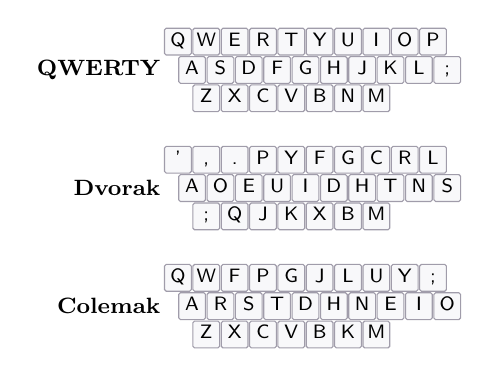
\begin{tikzpicture}
% Three keyboards stacked. Same 30 physical key positions; each layout
% reassigns the letters at those positions. Visual comparison highlights
% how a keymap is a re-binding of an unchanged physical substrate.
% Three keyboards stacked. Punctuation chars are wrapped in {} so
% TikZ's \foreach parser doesn't treat them as separators.
\foreach \layoutY/\name in {3.0/QWERTY, 1.5/Dvorak, 0.0/Colemak} {
 \node[anchor=east, font=\footnotesize\bfseries] at (-0.1, \layoutY+0.36) {\name};
}
% QWERTY rows
\foreach \l [count=\i] in {Q,W,E,R,T,Y,U,I,O,P}
 \node[kcap] at ({(\i-1)*0.36}, 3.72) {\strut\l};
\foreach \l [count=\i] in {A,S,D,F,G,H,J,K,L,{;}}
 \node[kcap] at ({(\i-1)*0.36+0.18}, 3.36) {\strut\l};
\foreach \l [count=\i] in {Z,X,C,V,B,N,M}
 \node[kcap] at ({(\i-1)*0.36+0.36}, 3.0) {\strut\l};
% Dvorak rows
\foreach \l [count=\i] in {{'},{,},{.},P,Y,F,G,C,R,L}
 \node[kcap] at ({(\i-1)*0.36}, 2.22) {\strut\l};
\foreach \l [count=\i] in {A,O,E,U,I,D,H,T,N,S}
 \node[kcap] at ({(\i-1)*0.36+0.18}, 1.86) {\strut\l};
\foreach \l [count=\i] in {{;},Q,J,K,X,B,M}
 \node[kcap] at ({(\i-1)*0.36+0.36}, 1.5) {\strut\l};
% Colemak rows
\foreach \l [count=\i] in {Q,W,F,P,G,J,L,U,Y,{;}}
 \node[kcap] at ({(\i-1)*0.36}, 0.72) {\strut\l};
\foreach \l [count=\i] in {A,R,S,T,D,H,N,E,I,O}
 \node[kcap] at ({(\i-1)*0.36+0.18}, 0.36) {\strut\l};
\foreach \l [count=\i] in {Z,X,C,V,B,K,M}
 \node[kcap] at ({(\i-1)*0.36+0.36}, 0) {\strut\l};
\end{tikzpicture}}
\caption{同一の物理的基体の上の三つのタイピング・キーマップ。各配列は同一のキー位置を異なる文字の集合へと再結合したものである。QWERTY（Sholes 1873年、一度も特許化されず）、Dvorak（Dvorak \& Dealey 1936年、US 2{,}040{,}248）、Colemak（Coleman 2006年、パブリックドメイン）。2010年以降のフォークの生態系がこの系を拡張している。}
\label{fig:typing-layouts}
\end{figure}

\section{系譜 II：楽器の配列}
\label{sec:lineage2}

楽器の配列は並行する歴史をたどってきた。Paul von Jankó の六列同型ピアノ鍵盤~\citep{janko1882}は Liszt と Rubinstein に支持され、Decker、Blüthner、Bösendorfer によって製造され、ニューヨークの Janko 音楽院で教えられた。採用のためのあらゆる社会的前提条件からすれば、それは標準的なピアノ鍵盤に取って代わるはずだった。そうはならなかった。現存することが知られている Janko ピアノは十台に満たない。Janko の事例は、社会的ソフトウェアとしてのキーマップという議論の負の極である。伝播のためのあらゆる条件が満たされながら、それでも伝播は失敗した。社会的ソフトウェアの契約が何であれ、それは支持と製造者と音楽院の総和以上のものである。

R.\ H.\ M.\ Bosanquet の一般化鍵盤~\citep{bosanquet1875generalized}は、53平均律（53-EDO）の異名同音ハーモニウムであり、また1875年の、48音のスキスマ的および4分の1コンマ中全音律のオルガンであって、1876年にサウス・ケンジントン博物館で実演された。それは本質的にあらゆる現代の同型コントローラの祖先である。Kaspar Wicki は1896年にバンドネオンのための同型音配列の特許を取得した~\citep{wicki1896}。コンサーティナ奏者の Brian Hayden は、1986年に本質的に同じ配列を独立に再発明し、再特許化した。九十年を隔てた二重の発明はそれ自体がひとつの議論である。この配列は\emph{発見}の性格をもっている——それが固有の文化的人工物だからではなく、音楽の根底的な構造がそれを有用にするがゆえに再帰する種類の対象なのである。

\begin{figure}[t]
\centering
\resizebox{0.88\columnwidth}{!}{%
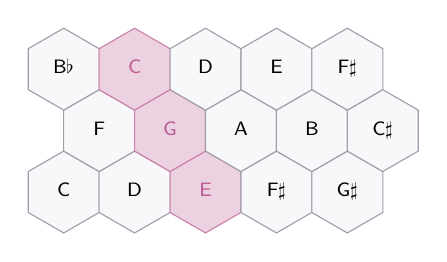
\begin{tikzpicture}
% Compact Wicki-Hayden-style hex schematic. Same-row neighbors
% differ by a whole tone; up-and-right neighbors differ by a P4.
% C major triad (C-E-G) highlighted; the same shape transposes to
% any key by translation across the surface ("isomorphism" claim).
% Hexes are EXPLICIT PATHS, not regular-polygon nodes — TikZ node
% sizing breaks the lattice. Pointy-top hexagon, circumradius R:
% width = sqrt(3)R, height = 2R. Tessellation: horizontal pitch =
% sqrt(3)R, row step = 1.5R, odd-row offset = sqrt(3)R/2.
\def\R{0.52}
\def\hexn#1#2#3{\begin{scope}[shift={(#1,#2)}]
 \draw[keystroke, fill=keyfill]
  (30:\R) -- (90:\R) -- (150:\R) -- (210:\R) -- (270:\R) -- (330:\R) -- cycle;
 \node[font=\scriptsize\sffamily, inner sep=0pt] at (0,0) {\strut#3};
\end{scope}}
\def\hexm#1#2#3{\begin{scope}[shift={(#1,#2)}]
 \draw[keymapped!70, fill=keymapped!25]
  (30:\R) -- (90:\R) -- (150:\R) -- (210:\R) -- (270:\R) -- (330:\R) -- cycle;
 \node[font=\scriptsize\sffamily, text=keymapped!90, inner sep=0pt] at (0,0) {\strut#3};
\end{scope}}
\def\hp{0.9006}  % horizontal pitch (sqrt(3) * R)
\def\vp{0.78}   % vertical pitch (1.5 * R)
\def\offx{0.4503} % horizontal offset for alternate rows (hp / 2)
% Row 0 (bottom)
\hexn{0}{0}{C}
\hexn{\hp}{0}{D}
\hexm{2*\hp}{0}{E}
\hexn{3*\hp}{0}{F$\sharp$}
\hexn{4*\hp}{0}{G$\sharp$}
% Row 1 (middle, offset)
\hexn{\offx}{\vp}{F}
\hexm{\offx + \hp}{\vp}{G}
\hexn{\offx + 2*\hp}{\vp}{A}
\hexn{\offx + 3*\hp}{\vp}{B}
\hexn{\offx + 4*\hp}{\vp}{C$\sharp$}
% Row 2 (top)
\hexn{0}{2*\vp}{B$\flat$}
\hexm{\hp}{2*\vp}{C}
\hexn{2*\hp}{2*\vp}{D}
\hexn{3*\hp}{2*\vp}{E}
\hexn{4*\hp}{2*\vp}{F$\sharp$}
\end{tikzpicture}}
\caption{Wicki--Hayden のヘクサゴナル配列（Wicki 1896年 / Hayden 1986年）。同じ列の隣接音は全音だけ異なり、右上の隣接音は完全四度だけ異なる。C 長三和音（$C\,E\,G$）が強調されている。和音は表面上の固定された三つのセルの形であり、その形を平行移動させることで和音を任意の調へ移調できる。「移調は平行移動である」が同型鍵盤の中心的主張であり、標準的なピアノの白鍵と黒鍵の非対称性が犠牲にする性質である。}
\label{fig:wicki}
\end{figure}

\begin{figure*}[t]
\centering
% Interval-signature bars (full text width). Each bar reads left to
% right as the sequence of intervals the instrument's layout steps
% through; every block is one interval, its WIDTH = its size in
% semitones and its COLOR fixed by the legend. A regular instrument
% is a row of equal blocks; an asymmetric one has a visible odd block.
\begingroup
\definecolor{iv1}{HTML}{E2574C}% m2 (1 semitone)
\definecolor{iv2}{HTML}{EE9B3A}% M2 (2)
\definecolor{iv3}{HTML}{D1A52A}% m3 (3) — darkened so white slice text reads
\definecolor{iv4}{HTML}{4FAE54}% M3 (4)
\definecolor{iv5}{HTML}{3A86D6}% P4 (5)
\definecolor{iv7}{HTML}{8A5CF6}% P5 (7)
\resizebox{\textwidth}{!}{%
\begin{tikzpicture}
\def\rad{1.55}
% \pie{xshift}{name}{deg-per-semitone}{ semitones/color/label, ... }
% Slices sweep clockwise from 12 o'clock; angle = semitones. A regular
% instrument is an even wheel; an asymmetric one has a visibly odd slice.
% list fields: semitones / fill / interval-label / note-label.
% The note sits INSIDE the slice (the actual open string, scale degree,
% or valve number); the interval name sits just outside the rim.
\def\pie#1#2#3#4{\begin{scope}[shift={(#1,0)}]
 \xdef\angA{90}
 \foreach \s/\c/\lab/\nt in {#4}{
  \pgfmathsetmacro\angB{\angA-\s*#3}
  \filldraw[fill=\c, draw=\c!55!black, line width=0.6pt]
   (0,0) -- (\angA:\rad) arc[start angle=\angA, end angle=\angB, radius=\rad] -- cycle;
  \pgfmathsetmacro\angM{(\angA+\angB)/2}
  \node[font=\large\sffamily\bfseries, text=white] at (\angM:{0.58*\rad}) {\nt};
  \node[font=\small\sffamily, text=acdark] at (\angM:{\rad+0.32}) {\lab};
  \xdef\angA{\angB}
 }
 \node[font=\normalsize\sffamily\bfseries, text=acdark] at (0,{-\rad-1.08}) {#2};
\end{scope}}
% --- legend ---
\begin{scope}[shift={(-0.4,3.15)}]
 \node[font=\small\sffamily\bfseries, text=acdark, anchor=west] at (0,0.28) {音程 \;(扇形の角度 $\propto$ 半音):};
 \def\lg#1#2#3{\draw[fill=#2, draw=#2!55!black, rounded corners=2pt] (#1,0.0) rectangle (#1+0.56,0.56);
  \node[font=\small\sffamily, text=acdark, anchor=west] at (#1+0.66,0.28) {#3};}
 \lg{7.7}{iv1}{m2}\lg{9.1}{iv2}{M2}\lg{10.5}{iv3}{m3}\lg{11.9}{iv4}{M3}\lg{13.3}{iv5}{P4}\lg{14.7}{iv7}{P5}
\end{scope}
% --- four wheels in a row ---
\pie{0}{Guitar \textperiodcentered\ EADGBE}{15}{5/iv5/P4/E, 5/iv5/P4/A, 5/iv5/P4/D, 4/iv4/M3/G, 5/iv5/P4/B}
% emphasize the guitar's lone M3 wedge (starts -135, spans 60 deg)
\draw[keymapped, line width=1.5pt]
 (0,0) -- (-135:\rad) arc[start angle=-135, end angle=-195, radius=\rad] -- cycle;
\pie{4.7}{Violin \textperiodcentered\ GDAE}{17.142857}{7/iv7/P5/G, 7/iv7/P5/D, 7/iv7/P5/A}
\pie{9.4}{Trumpet \textperiodcentered\ 3 valves}{60}{2/iv2/M2/1, 1/iv1/m2/2, 3/iv3/m3/3}
\pie{14.1}{Ocarina \textperiodcentered\ diatonic}{30}{2/iv2/M2/C, 2/iv2/M2/D, 1/iv1/m2/E, 2/iv2/M2/F, 2/iv2/M2/G, 2/iv2/M2/A, 1/iv1/m2/B}
\end{tikzpicture}}
\endgroup
\caption{\emph{音程ホイール}として読まれる四つの非対称な音高インターフェース。各ホイールは、その配列が組み立てられている音程の系列を時計回りに掃く。各扇形はひとつの音程であり、その角度は半音での大きさによって定まり、その色は凡例によって固定される。規則的な楽器は均等なホイールであり、非対称な楽器は目に見えて奇妙な扇形をひとつ担う。ギターの EADGBE は完全四度の環であり、G と B のあいだの長三度（輪郭で示す）によって一度だけ破られている——標準的な和音の形を手の下に収め、フォーク、ブルース、ジャズ、ロックのギターがそれに対して書かれてきた、その不規則性である。ヴァイオリンは三つの同一の完全五度であり、完全に均等なホイールでありながら、各開放弦はそれぞれ異なる絶対音高をもつ。トランペットの三つのバルブは音高を二、一、三半音だけ下げる——設計によってすべて異なり、その組み合わせがあらゆる半音階の段に到達する。オカリナは全音階それ自身のホイールであり、五つの長い段のあいだに二つの短い段がある。標準的なピアノも同じ一族に属する——多くの表面に体現された全音階の命名キーマップであり、それぞれが独自の非対称性をもっている。}
\label{fig:asymmetric-instruments}
\end{figure*}

これらの表面のそれぞれが独自の系譜を担っている。三バルブのトランペット（Stölzel と Blühmel、1814年頃）は、一世紀にわたるナチュラル・トランペットの実践ののちに標準化され、ウィーン式とロータリー式のバルブの変種がそれぞれ独自の音高上のキーマップを構成している。オカリナはメソアメリカの容器笛から、1853年に Budrio で Giuseppe Donati が行った標準化へと至り、そこでは非対称な指孔の配置が10孔のパターンを教えられるものにした。ギターの EADGBE 調弦は、1700年代にリュートの調弦から結晶化した。B 弦の不規則性が、それ以外は均一な四度を破ることで、開放和音の形が手の下に収まるようになり、フォーク、ブルース、ジャズ、ロックのギターの文献全体が、その単一の不規則な音程に対して書かれてきた。ヴァイオリンの厳密な完全五度（G\,D\,A\,E）は、管弦楽のレパートリーがそれに対して書かれている、五度に基づく弦楽セクションの慣習を支えている。いずれの場合も、非対称性は音楽が許容する欠陥ではなく、音楽がそのまわりに書かれてきた遺産である——それは初心者が最初に何を学ぶか、練習曲がどのようなものになるか、どの記法が旅をしたかを定める。標準的なピアノ鍵盤はこの伝統の内側に位置するのであって、その上にあるのではない。同型の代替案は、それらが時として認めるよりも根本的な何かを提案している。すなわち、これらすべての楽器の一族を互いに結びつけている、音高命名のキーマップの解体である。

Jankó の失敗——そしてより広く Wicki--Hayden／ヘクサゴナル格子の一族の周縁性——についての標準的な読みは、David--Liebowitz モデルにおける経路依存性である。ピアノはロックインだけによって存続している。より手強い読みもありうる。標準的なピアノ鍵盤の白鍵と黒鍵の非対称性は、半音階円のランドマーク地図である——奏者は $C$ が二つの黒鍵の左にあるからその位置を知る——絶対的な音高の位置を記憶から目と手へと外部化している。非対称性を剥ぎ取れば、外部化された情報には着地する場所がなくなる。移調は平行移動になるが、絶対的な位置は想起になる。四世紀のレパートリーがこの非対称性を\emph{調性格}へと吸収してきた——$F^\sharp$ 長調の運指は $C$ 長調のそれとは異なり、音楽はその差異に対して書かれてきた——ので、「歴史の偶然」を取り除くことは、文献がそれに沿って書かれてきた意味の一軸を平坦化してしまう。これは経路依存性の物語を解消するというよりも、それを反対側から切り開く。ピアノは経路依存的で\emph{あり}、しかもその経路は、その代替案と厳密には等価でない対象を生み出した。より深い手は、西洋の調性体系それ自体をひとつのキーマップとして扱うことである。七文字の全音階命名 $C\,D\,E\,F\,G\,A\,B$ は、すでに音高空間にわたる社会的ソフトウェアの契約であり、理論、教育法、そしてあらゆる調号のなかに書き込まれている。ピアノの白鍵はそのキーマップの物理的な実現であり、黒鍵は記法がすでに $\sharp$ と $\flat$ で名づけている変化である。したがって標準的なピアノは二つの仕事を一度にこなしている——物理的なインターフェースと記法的な符号化である——そして同型の代替案は、第一のものを最適化するために第二のものを解体することを提案している。この議論は、音高を全音階の文字で命名する12平均律のレパートリーに限定される。それの外では——19、22、31、53-EDO のゼノハーモニックな音楽、マカームやその他の異なる音高命名キーマップをもつ調性体系では——ピアノは積極的に妨げとなり、Bosanquet から Lumatone へと至る同型の系には、レパートリーに根ざした強い主張がある。その範囲の内側では、同じ音高命名のキーマップこそが \texttt{notepat.com}（\textsection\ref{sec:notepat}）が保存するものであり、QWERTY の文字キャップの上に運ばれ、文字 \texttt{C} を押すと音 $C$ が鳴る。Jankó が物理的なインターフェースを最適化するために命名キーマップを解体し、半音階階段の DAW 慣習が\emph{両方}を解体する（\textsection\ref{sec:daw}）のに対して、\texttt{notepat.com} は命名の契約を変えずに保ち、Sholes の1873年の機械工たちが問うた問いだけを再び問う——どの物理的な表面がそれを未来へ運ぶべきか、という問いを。

現代の子孫は商業製品である——C-Thru AXiS-49（2008年）~\citep{cthru2008axis49}、Jim Plamondon の Thummer~\citep{plamondon2003thummer}、Roger Linn の LinnStrument、ROLI Seaboard、Lumatone のヘクサゴナル格子、そして Lippold Haken の Continuum Fingerboard~\citep{haken1998indiscrete}。Andrew Milne、William Sethares、James Plamondon による同型コントローラと調律連続体についての論文~\citep{milne2007isomorphic,milne2008tuning}が理論的基盤を提供している。社会的ソフトウェアとしてのキーマップという視点から際立つのは、これらの楽器が\emph{設定可能な状態で出荷される}ことである。配列はユーザーがアップロードする明示的な対象であり、ゼノハーモニックの共同体は配列をファイルとして共有する。とりわけ Lumatone はキーマップを配布の単位として扱う。楽器は基体であり、キーマップこそがそれを音楽的にする人工物である。

\section{半音階階段、すなわち AWSED：所有なき収束}
\label{sec:daw}

社会的ソフトウェアとしてのキーマップという議論にとって最も強力な現代の事例は、すべての主要なデジタル・オーディオ・ワークステーションが共有する、事実上の半音階階段状の QWERTY ピアノのキーマップである。Ableton Live、Logic Pro、GarageBand、FL Studio はすべて、同じ慣習を既定で出荷している~\citep{ableton_musical_typing,apple_logic_musicaltyping,imageline_typing_piano}。この慣習の形はこうである——QWERTY キーボードの下の三列を取り、ある一列を、C から上昇する半音階の白鍵として扱い、その上の列を、ピアノで黒鍵が落ちるはずの隙間における黒鍵として扱う。Ableton、Logic、GarageBand は、白鍵 $C\,D\,E\,F\,G\,A\,B\,C$ にホーム列 \keys{A,S,D,F,G,H,J,K} を、黒鍵 $C^\sharp\,D^\sharp\,F^\sharp\,G^\sharp\,A^\sharp$ にその上の列 \keys{W,E,T,Y,U} を用いる。FL Studio は下のオクターブの白鍵に最下列 \keys{Z,X,C,V,B,N,M} を用い、黒鍵には同じ上列のパターンを用いる。原理は同一である。正確な列の割り当てが一列ぶん異なる。

この慣習は三十年にわたって名もなく伝播してきた。本稿は、それを研究すべき分野のために、ここでそれに名を与える——最初の五つの半音階音のキーを、$C$ が \key{A}、$C^\sharp$ が \key{W}、$D$ が \key{S}、$D^\sharp$ が \key{E}、$E$ が \key{D} と、音高の順に読めば、それらは \textbf{AWSED} と綴られる。\emph{以後これを AWSED 配列と呼ぶ}（ホーム列の変種。FL Studio の変種はその最下列への移調である）。この名は、以下で論じる PC ゲームの移動慣習である WASD と韻を踏むように選ばれている。両者は構造的に同じ対象——誰も設計せず誰もが出荷する、所有者なき、仕様化されていない、アプリケーション横断的な入力キーマップ——であり、この韻こそが議論である。WASD はその共同体によって名づけられ、教えられ、正典化された。AWSED はそもそも名づけられすらしなかった。それこそが、それが研究を逃れてきた理由にほかならない。名のない物は見えにくく、批評しにくく、引用することが不可能である。それに名づけることが最初の手である。

誰もこの慣習を設計しなかった。どの仕様もそれを定義しない。統治機関も、保守者も、資金調達の仕組みもない。この慣習が存在するのは四つの実装が一致するからであり、四つの実装が一致するのは、その慣習が現代の DAW に先立つ1990年代のトラッカー・ソフトウェア（FastTracker、Renoise、Impulse Tracker）にすでに存在していたからであり、また、ひとつの DAW を学んだすべてのユーザーが次のものも同じように振る舞うことを期待するからである。ある DAW のために書かれたチュートリアル文書は、多かれ少なかれ別の DAW へと移し替えられる。これは\emph{社会的ソフトウェアの契約}の最も純粋な形である——中央の権威をもたずに、教育法と期待を通して伝播する、版管理された仮想的対象である。

\begin{figure}[t]
\centering
\resizebox{\columnwidth}{!}{%
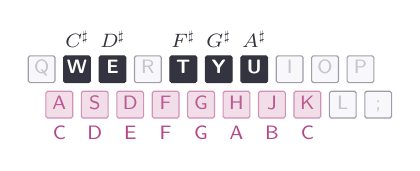
\begin{tikzpicture}
% Upper QWERTY row (sharps in DAW chromatic-staircase). Only 5 keys
% are mapped (W E T Y U); R and I sit in the gaps with no note.
\foreach \l/\note/\mapped [count=\i] in {%
 Q/{}/0, W/$C^\sharp$/1, E/$D^\sharp$/1, R/{}/0, T/$F^\sharp$/1,
 Y/$G^\sharp$/1, U/$A^\sharp$/1, I/{}/0, O/{}/0, P/{}/0%
}{
 \ifnum\mapped=1
  \node[kcap sharp] (k\i) at ({(\i-1)*0.45}, 1.8) {\strut\l};
  \node[font=\scriptsize\sffamily, text=keysharp, anchor=south, inner sep=1pt]
   at ({(\i-1)*0.45}, 2.03) {\note};
 \else
  \node[kcap, text=keystroke!60] (k\i) at ({(\i-1)*0.45}, 1.8) {\strut\l};
 \fi
}
% Home row (whites). 8 of 10 keys mapped (A through K = C..C).
\foreach \l/\note/\mapped [count=\i] in {%
 A/C/1, S/D/1, D/E/1, F/F/1, G/G/1, H/A/1, J/B/1, K/C/1, L/{}/0, {;}/{}/0%
}{
 \ifnum\mapped=1
  \node[kcap mapped] at ({(\i-1)*0.45+0.225}, 1.35) {\strut\l};
  \node[font=\scriptsize\sffamily, text=keymapped, anchor=north, inner sep=1pt]
   at ({(\i-1)*0.45+0.225}, 1.12) {\note};
 \else
  \node[kcap, text=keystroke!60] at ({(\i-1)*0.45+0.225}, 1.35) {\strut\l};
 \fi
}
\end{tikzpicture}}
\caption{AWSED 配列——DAW の半音階階段状の QWERTY ピアノのキーマップ（Ableton、Logic、GarageBand の変種）。ホーム列 \texttt{A~S~D~F~G~H~J~K} は白鍵 $C$ から $C$ までを鳴らす。その上の列は、ピアノの黒鍵が落ちるはずの隙間にシャープを置く（$C^\sharp\,D^\sharp$、続いて \texttt{R} に隙間、$F^\sharp\,G^\sharp\,A^\sharp$、続いて隙間）。名は最初の五つの半音階音 $C\,C^\sharp\,D\,D^\sharp\,E$ に由来し、それらは \key{A}\,\key{W}\,\key{S}\,\key{E}\,\key{D} に落ちる。各キャップ上の QWERTY の文字は、それが生み出す音名とは何の関係もない。}
\label{fig:daw-staircase}
\end{figure}

それはまた、本稿が論じるところでは、まずく設計されている。AWSED 配列には三つの構造的な弱点がある。\textbf{第一に}、各キー上の QWERTY の文字は、それが生み出す音名とは何の関係もない。\key{A} は C を、\key{S} は D を、\key{D} は E を鳴らす（図~\ref{fig:daw-staircase}）。西洋の七音音階を学んだユーザーは、その知識からキーマップへの手がかりを何ら得られない。\textbf{第二に}、それはただひとつのオクターブ（$C$ から $C$）しか提供しないのに、そのひとつのオクターブをホーム列全体にわたって、\key{A} から \key{K} まで——\emph{両}手が置かれる幅いっぱい——に広げる。それは片手のためのコンパクトなオクターブでもなければ、生産的な両手の音域でもない。両手ぶんのキーボードを費やしてただひとつのオクターブを生み出し、そこで止まる。幅は両手のために配置されているのに、音域は片手のために寸法取りされている。\textbf{第三に}、このキーマップはチュートリアルなしには読み解けない。記憶の手がかりはなく、物理的なキーに印刷された図もなく、第一原理から写像を導く方法もない。手引書を必要とするキーマップは、その社会的ソフトウェアの性格を失ったキーマップである。

この命名は無意味なものではなかった。その自然な対照は、PC ゲームにおける移動慣習である WASD である——そしてこのほぼアナグラムは、偶然というよりむしろひとつの診断である。WASD は AWSED と同じ構造的な形——所有者なき、仕様化されていない、アプリケーション横断的なユーザー入力の慣習——をもつが、伝播の歴史が異なる。WASD 以前、PC ゲームは既定で矢印キーを用いていた（Wolfenstein 3D、Doom、1997年までの Quake シリーズ）~\citep{wikipedia_arrow_keys}。中間的な実験には System Shock の ASDX（1994年）や Descent の AZ+QE が含まれる。競技 Quake プレイヤーの Dennis ``Thresh'' Fong は、自費出版した設定ガイド~\citep{thresh_quake_bible}を通して WASD 配列を普及させ、1997年に最初の全国規模の Quake トーナメントで優勝した。Valve の Half-Life は1998年に WASD を既定として出荷し、2000年代初頭までにこの慣習は PC ゲームを飽和させた~\citep{fenlon2016wasd}。WASD が存続するのは、DAW の半音階階段にはない理由による。それは公式の既定よりも純粋に優れているのである。それは右手をマウスのために解放し、Shift／Space／Ctrl／Tab に隣接し、QWERTY キーボード上のホーム列の指の配置を活用する。構造的な教訓は、伝播が社会的媒介\emph{と}適応度の関数であるということである。WASD が伝播したのは、Fong の教育法がプレイヤーに届き、\emph{かつ}その写像が実力で勝ったからである。半音階階段は教育法だけで伝播した——実力はその逆を走っていたにもかかわらず。両方の事例は同じ範疇に属する——アプリケーションを横断してユーザー入力を統べる、所有者なき慣習である。それらは、この範疇が、よく設計されたものとまずく設計されたもの、ユーザーに検証されたものと惰性によって継承されたものの両方にまたがるほど大きいことを示している。

\section{Notepat.com：自らの名を名乗る音符}
\label{sec:notepat}

この既存の慣習に対して、\texttt{notepat.com} は異なるキーマップを提案する（図~\ref{fig:notepat-keymap}）。設計原理はただひとつである——\emph{自らの名を名乗る音符}。QWERTY の文字 \key{C} は C を鳴らす。QWERTY の文字 \key{D} は D を鳴らす。西洋音階の七つの幹音——$C\,D\,E\,F\,G\,A\,B$——は、その文字が名づける音を鳴らす。上のオクターブはアルファベット順に続く——$C_5\,D_5\,E_5\,F_5\,G_5\,A_5\,B_5$ に \keys{H,I,J,K,L,M,N}。シャープは、QWERTY の文字が許すところでは、ピアノの黒鍵になぞらえて、対応する幹音の一段上の列に置かれる——$C^\sharp\,D^\sharp\,F^\sharp\,G^\sharp\,A^\sharp$ に \keys{V,S,W,R,Q}。下のオクターブは左手の下に、上のオクターブは右手の下に落ちる。

このキーマップは AWSED の三つの弱点のそれぞれを反転させる。\textbf{第一に}、各キー上の文字が音名そのもの\emph{である}。西洋音階を知る者なら誰でも、すでにこのキーマップを知っている。\textbf{第二に}、それは両手の幅を生産的に費やす。左手が下のオクターブを弾き、右手が上でそれを鏡映するので、AWSED がひとつのオクターブに費やすのと同じ幅が二つのオクターブを生む。\textbf{第三に}、このキーマップは自己文書化されている。図~\ref{fig:notepat-keymap} の図は、「CDEFGAB」と綴れる者なら誰でも記憶から再現できる。

三つのことが \texttt{notepat.com} を本稿のキーマップのなかで異例なものにしている——それは名をもち（多くは、AWSED（\textsection\ref{sec:daw}）のように、名をもたなかった）、その音符が自らの名を名乗るのでキーマップが自らを指し示し、そしてすでに多くの実装で動いている。\texttt{notepat.com} の貢献は実装ではない。実装は、設計上、控えめである——キーボードのイベントを音声合成 API へと振り分ける、数百行の JavaScript である。貢献はキーマップである。それは五つの実装にわたって提示される——\texttt{notepat.com} のウェブ・ピース、AC Native OS のベアメタル移植、MenuBand の macOS メニューバー・アプリ、Ableton（Max for Live）プラグイン、そして \texttt{babypat}——そしてキーマップこそが、それらすべてにわたって同一である唯一のものである。音符命名の記法は楽器よりもさらに遠くまで旅をする。それは AC の分散シーケンサ \texttt{clock} で再利用され、そこでは同じ一文字の音高がネットワーク化された再生を駆動する。それは \texttt{notepat.com} の形をした社会的ソフトウェアの契約である。

実装を並べて比較する読者は、キーが図~\ref{fig:notepat-keymap} の表を超えたことをしているのに気づくだろう。AC Native と MenuBand では、\texttt{Space} を押し続けると、実際の音声出力の直近数秒を逆再生する。ウェブ・ピースと AC Native では、音を打ちながら \texttt{Shift} を押し続けると、その声部が離されたときに長い減衰の尾を得る。\texttt{Enter} を押し続けるとその声部が無限に保たれ、\texttt{Backspace} は保たれたすべての声部を消去する。MenuBand と AC Native では、\texttt{Control}、\texttt{Alt}、そしてその二つをともに用いると、一回の打鍵が長三和音、短三和音、あるいは保留和音へと昇格される。これらのいずれもキーマップの図には現れず、その省略は意図的である。これらのバインドは\emph{拡張的な演奏層}を形づくり、その層と音高写像とのあいだの線こそが、社会的ソフトウェアの契約それ自体の境界である（表~\ref{tab:contract-line}）。

\begin{table}[t]
\footnotesize
\setlength{\tabcolsep}{3pt}
\renewcommand{\arraystretch}{1.05}
\centering
\caption{契約線で分けられた \texttt{notepat.com} のバインド。線の上：すべての実装にわたって同一である音高写像——社会的ソフトウェアの対象。線の下：各基体が自由に異なってよい拡張的な演奏層。}
\label{tab:contract-line}
\begin{adjustbox}{max width=\linewidth,center}%
\begin{tabularx}{\linewidth}{@{}>{\RaggedRight}p{0.30\columnwidth}>{\RaggedRight}X>{\RaggedRight\arraybackslash}p{0.21\columnwidth}@{}}
\toprule
\textbf{バインド} & \textbf{意味} & \textbf{場所} \\
\midrule
\multicolumn{3}{@{}l}{\emph{音高の契約}} \\[0.1em]
\texttt{C D E F G A B} & 幹音 $C_4$--$B_4$、左手 & すべて \\
\texttt{H I J K L M N} & 幹音 $C_5$--$B_5$、右手 & すべて \\
\texttt{V S W R Q} & シャープ、一段上の列 & すべて \\
\midrule
\multicolumn{3}{@{}l}{\emph{拡張的な演奏層}} \\[0.1em]
\texttt{Shift}（保持） & 持続：長い減衰の尾 & ウェブ、Native \\
\texttt{Enter}（保持） & 声部を保つ；\texttt{Backspace} で消去 & ウェブ、Native \\
\texttt{Space}（保持） & 直近の音声を逆再生 & Native、MenuBand \\
\texttt{Ctrl}\,/\,\texttt{Alt}\,/\,両方 & 長／短／sus2 三和音 & MenuBand、Native \\
\texttt{<}~\texttt{>} & 手ごとのオクターブ移動 & ウェブ \\
\bottomrule
\end{tabularx}%
\end{adjustbox}
\end{table}

表~\ref{tab:contract-line} の二つの半分は、異なる規則によって統べられている。線の上では、逸脱は破綻である。\texttt{C} を音 $C$ から再写像する実装は、\texttt{notepat.com} の移植ではなく別の楽器になるだろう。線の下では、逸脱は語法である。各基体は、その身体が可能にする身振りを育てる。機械全体を所有するベアメタル OS は、自らの音声出力をリングバッファに収め、それを逆向きに再生できる。システム全体のイベントタップに乗るメニューバー・アプリは、修飾キーの和音に頼る。ブラウザのタブに住むウェブ・ピースは、持続させ、保持する。ユーザーはこれらの差異を破綻としては経験せず、どの実装も他の実装の身振りを担う義務はない。同じ二層構造はより古い事例にも見える。契約としての QWERTY はメディアキーや \texttt{Fn} 層について何も語らず、それらはベンダーごとに自由に異なるが、誰も ThinkPad を QWERTY のフォークとは呼ばない。Vim の中核的な移動は契約であり、プラグインのバインドは語法である。このことが示唆するのは、キーマップとは、ある実装が出荷するすべてのバインドの集合ではない、ということである。それは、その改変を共同体が同一性の侵害として経験するであろう部分集合である——そして、あるバインドが線のどちら側に落ちるかについての実践的な一つの試金石は、記法という表面（\textsection\ref{sec:notation}）がそれを担うかどうかである。\texttt{C D E F G A B} はテキストとして旅をする。「時間を逆転させるためにスペースを押し続ける」は、各移植において実演によって再び教えられねばならない、基体ごとの身振りである。

これこそが、本稿が読者に見てもらいたい手である。支配的な DAW の半音階階段のキーマップは決して\emph{選ばれた}ものではなかった——それはトラッカー・ソフトウェアから\emph{継承され}、ユーザーの期待によって存続し、アプリケーション横断的な慣習によってロックインされた。\texttt{notepat.com} は、その余地が開かれていることを示している。すなわち、意図的に設計された代替案を、ひとりの開発者が数百行のコードで著すことができ、一年のうちに複数の実装にわたって出荷し、競合する社会的ソフトウェアの契約としてより広い共同体に提供できるのである。政治的な賭けは、いかなる単一の事例においても小さく、総体としては大きい——\emph{その余地はあらゆるところで開かれている}。

\section{記法：言説の表面}
\label{sec:notation}

ここまでの議論はキーマップを表として扱ってきた。しかしキーマップは表であるだけではない。それはまた\emph{記法}——そのキーマップの使用が読まれ、書かれ、教えられ、引用され、論じられるテキストとしての形式——をもつ。記法はキーマップの言説の表面である。それはまた、本稿が論じるところでは、実際に旅をするキーマップの半分である。記法が可搬であるキーマップはテキストとして伝播し、記法がぎこちないか欠けているキーマップは筋肉の記憶としてのみ伝播する。したがって記法の質は、キーマップの設計可能な性質であって、派生的な人工物ではない。バインドの表だけを出荷する設計者は、対象の半分しか出荷していない。

典型的な事例は Vim である。Vim の根底にあるキーマップは、打鍵をエディタのコマンドに対応づける表である——\texttt{d} は削除演算子を、\texttt{i} は内側のテキスト・オブジェクトを、\texttt{w} は単語の移動を開始する。しかし Vim の言説で旅をするのはその表ではない。旅をするのは\emph{記法}である——\texttt{dd}、\texttt{ciw}、\texttt{gg}、\texttt{:wq}、\texttt{<C-w>}（図~\ref{fig:vim-modes}）。チュートリアル、ブログ記事、README ファイル、vimtutor、そして長く続く vim 対 emacs の論争は、すべてこの記法で行われる。この記法はきわめて可搬であり、Vim の外でもそのまま生き残る——\emph{vim モード}は Visual Studio Code に、JupyterLab に、\texttt{set -o vi} を介してシェルに、macOS の Cocoa テキストフィールドに、Vimium を介してブラウザに現れる。移植されているのは記法である。ランタイムは偶有的である。

\begin{figure}[t]
\centering
\begin{tikzpicture}[
 modebox/.style={draw=keymapped!70, fill=keymapped!12,
          rounded corners=2pt, minimum width=1.6cm,
          minimum height=0.6cm, font=\small\sffamily,
          text=keymapped!90, inner sep=2pt},
 arrow/.style={-{Stealth[length=4pt,width=4pt]}, draw=keystroke!90,
         line width=0.5pt},
 cmd/.style={font=\footnotesize\ttfamily, text=acdark}
]
% Three Vim modes wired by their command-notation transitions.
\node[modebox] (normal) at (0, 0) {NORMAL};
\node[modebox] (insert) at (3.0, 0) {INSERT};
\node[modebox] (visual) at (-3.0, 0) {VISUAL};
\draw[arrow] ([yshift=4pt]normal.east) -- node[above, cmd] {\texttt{i}\,/\,\texttt{a}\,/\,\texttt{o}} ([yshift=4pt]insert.west);
\draw[arrow] ([yshift=-4pt]insert.west) -- node[below, cmd] {\texttt{<Esc>}} ([yshift=-4pt]normal.east);
\draw[arrow] ([yshift=4pt]normal.west) -- node[above, cmd] {\texttt{v}\,/\,\texttt{V}\,/\,\texttt{<C-v>}} ([yshift=4pt]visual.east);
\draw[arrow] ([yshift=-4pt]visual.east) -- node[below, cmd] {\texttt{<Esc>}} ([yshift=-4pt]normal.west);
% A row of canonical commands underneath
\node[font=\footnotesize\ttfamily, text=acdark, anchor=north] at (0, -1.0)
 {\texttt{dd}\,\,\texttt{ciw}\,\,\texttt{gg}\,\,\texttt{:wq}\,\,\texttt{<C-w>v}\,\,\texttt{y2}\$};
\end{tikzpicture}
\caption{Vim のモード式キーマップとその旅をする記法。モード（NORMAL、INSERT、VISUAL）はラベル付きの打鍵による遷移で接続されている。よく使われるコマンド（\texttt{dd} 行削除、\texttt{ciw} 内側の単語の変更、\texttt{gg} 先頭へ、\texttt{:wq} 保存して終了、など）がキーマップの言説的な通貨である。この記法はきわめて可搬であり、VS~Code、JupyterLab、Vimium、macOS の Cocoa テキストシステム、そして \texttt{set -o vi} に再実装されている。}
\label{fig:vim-modes}
\end{figure}

DAW の半音階階段は負の事例である。それには可搬な記法がない。Ableton のミュージカル・タイピングで弾かれた旋律を書くには、出来事の系列の散文——「\key{A} を押し、次に \key{S}、次に \key{D}」——に頼るほかなく、それは音楽ではなく入力を記述している。これを Singmaster のキューブ記法~\citep{singmaster1981notes}（図~\ref{fig:singmaster}）と比べてみよ。そこでは \texttt{R U R' U' R U2 R'} が、ルービックキューブのアルゴリズムをキューバーのあいだで損なわれることなく旅させる。あるいはナッシュビル・ナンバー・システム~\citep{matthews1984nashville,williams1988nashville}と比べてみよ。そこでは「1--4--5」が和音進行をセッション・ミュージシャンのあいだで旅させる。あるいは Plover ステノ理論~\citep{knight2010plover}と比べてみよ。そこでは和音の記法が、速記のパターンを共同体が編集する辞書を通して旅させる。DAW の階段にはそのような取っ手がない。そのキーは物理的な位置によってしか指し示せない。したがってこのキーマップは筋肉の記憶のなかに存在し、紙の上にはまれにしか存在しない——それこそが、おそらくより大きなユーザー基盤をもちながら、Vim よりも言説上の存在感が低い理由である。

\begin{figure}[t]
\centering
\resizebox{0.62\columnwidth}{!}{%
\begin{tikzpicture}
% Symmetric bounding box around the cube body (x=0) so \centering
% lands it centered --- the quarter-turn arrow otherwise extends the
% natural box rightward and pulls the cube off-center.
\useasboundingbox (-1.85,-2.55) rectangle (1.85,1.55);
% Isometric Rubik's cube, three visible faces: U (top), F (front-
% left), R (right). Faces are explicit-path parallelogram grids built
% from iso axes er=(0.866,0.5)s (right-up), el=(-0.866,0.5)s
% (left-up), ed=(0,-1)s (down), all meeting at the shared front-top
% vertex at the origin. The R face is tinted with a quarter-turn
% arrow: the diagram shows the first move of the algorithm below.
\def\s{0.55}
% Top face U: cells spanned by er and el
\foreach \i in {0,1,2} \foreach \j in {0,1,2}
 \draw[keystroke, fill=keyfill]
  ({0.866*\s*(\i-\j)}, {0.5*\s*(\i+\j)})
  -- ++({0.866*\s}, {0.5*\s})
  -- ++({-0.866*\s}, {0.5*\s})
  -- ++({-0.866*\s}, {-0.5*\s}) -- cycle;
% Front-left face F: cells spanned by el and ed — green stickers
\foreach \i in {0,1,2} \foreach \j in {0,1,2}
 \draw[acgreen!75!black, fill=acgreen!55]
  ({-0.866*\s*\i}, {0.5*\s*\i - \s*\j})
  -- ++({-0.866*\s}, {0.5*\s})
  -- ++(0, {-\s})
  -- ++({0.866*\s}, {-0.5*\s}) -- cycle;
% Right face R: cells spanned by er and ed — red stickers (mid-turn)
\foreach \i in {0,1,2} \foreach \j in {0,1,2}
 \draw[red!70!black, fill=red!55]
  ({0.866*\s*\i}, {0.5*\s*\i - \s*\j})
  -- ++({0.866*\s}, {0.5*\s})
  -- ++(0, {-\s})
  -- ++({-0.866*\s}, {-0.5*\s}) -- cycle;
% Face labels at face centers — standard sticker scheme:
% white up, green front, red right.
\node[font=\small\sffamily\bfseries, text=acdark]
 at (0, {1.5*\s + 0.5*\s}) {U};
\node[font=\small\sffamily\bfseries, text=white]
 at ({-0.866*\s*1.5 - 0.433*\s}, {0.75*\s - 1.5*\s + 0.25*\s}) {F};
\node[font=\small\sffamily\bfseries, text=white]
 at ({0.866*\s*1.5 + 0.433*\s}, {0.75*\s - 1.5*\s + 0.25*\s}) {R};
% Quarter-turn arrow for R: curved arrow hugging the right face's
% outer edge, pointing upward (clockwise as seen from the right).
\draw[-{Stealth[length=5pt,width=5pt]}, line width=1.1pt, red!70!black]
 ({0.866*\s*3.45}, {0.5*\s*3.45 - 2.5*\s})
 to[bend right=42]
 ({0.866*\s*3.45}, {0.5*\s*3.45 - 0.35*\s});
% Notation row underneath
\node[font=\small\ttfamily, anchor=north, text=acdark]
 at (0, {-3.2*\s}) {R\,U\,R$'$\,U$'$\,R\,U2\,R$'$};
\node[font=\scriptsize\sffamily, anchor=north, text=keystroke]
 at (0, {-4.0*\s}) {7手のアルゴリズム};
\end{tikzpicture}}
\caption{Singmaster のキューブ記法~\citep{singmaster1981notes}。各大文字がひとつの面を名づける（\textsf{U}p 上、\textsf{D}own 下、\textsf{L}eft 左、\textsf{R}ight 右、\textsf{F}ront 前、\textsf{B}ack 後）。裸の文字は時計回りの90度回転、プライム付きの文字（$\,'$）は反時計回りの90度回転、数字の2は180度回転である。七つのトークンの列 \texttt{R U R$'$ U$'$ R U2 R$'$} は、キューバー、GitHub リポジトリ、YouTube チュートリアルのあいだで可搬な、完全なアルゴリズムである——テキストとして旅をするキーマップと記法の対である。各面は標準的なステッカーの配色を担う（白が上、緑が前、赤が右）。\textsf{R} は90度回転の途中で描かれている——このアルゴリズムの最初の手である。}
\label{fig:singmaster}
\end{figure}

\texttt{notepat.com} の「音符が自らの名を名乗る」設計は、構造的な副次効果として、学ぶのに何の費用もかからない記法をもつ。notepat.com の系列を書くには、\texttt{C D E F G A B} と書く——それはまた標準的な音楽記法でもある。記法は \texttt{notepat.com} のために発明されたのではなく、既存のリテラシーから\emph{継承された}ものである。notepat.com のキーマップを一度も見たことのないピアニストでも、notepat.com のスコアを読むことができる。逆に、キーマップを学ぶ notepat.com の演奏者は、標準的な音高文字のリテラシーをも練習していることになる。これこそが、よく設計された記法の表面の姿である。記法が先行する知識からあまりに自明に導けるので、記法を学ぶのに何の費用もかからない。対照的に、Ableton の半音階階段は、notepat 風のスコアを \texttt{A S D F G H J} として再符号化することを要求するだろう——ひとつのキーマップに結びつけられた、他のどこでも役に立たない私的な記法である。

キーボードのショートカット採用についての経験的な文献は、この読みを裏づける。Peres らは、他のショートカット利用者と並んで働くことが、計算機経験単独よりも強いショートカット利用の予測因子であることを見いだした~\citep{peres2004shortcut}。Lozhkina らはこの結果を拡張する——ショートカットの発見の経路は対人的かつ視覚的である~\citep{lozhkina2025discovery}。Wang らは、ショートカットの設計がユーザーに手渡すものを名づけるために、明示的に\emph{語彙}という用語を用いる~\citep{wang2020keymap}。本稿の議論はこれらの知見を鋭くする。社会的媒介は他のユーザーのそばにいることの一般的な効果ではない。それは記法という表面を介した特定の伝達である。同僚は互いの画面を読み、\texttt{:wq} を見て、尋ね、学ぶ。伝達可能な記法がないところには、媒介すべき社会的媒介もない。同じ論理が、ライブコーディングのミニ記法の成功を説明する——Alex McLean と Geraint Wiggins の TidalCycles パターン言語~\citep{mclean2010tidal}、それを JavaScript へ移植した Strudel~\citep{roos2023strudel}、そしてライブコーディングされる映像のための Olivia Jack の Hydra 変換連鎖~\citep{jack2018hydra}、さらにはフォーク音楽のための ABC 記法~\citep{walshaw_abc}。いずれの場合もランタイムは偶有的である——Haskell、JavaScript、WebGL、MIDI プレイヤー——が、記法がその実践をランタイム、ワークショップ、数十年を越えて運ぶ。

\textsection\ref{sec:corollaries} の系の目録は、このレンズを通して読むと、ほとんどすべてが記法の目録である。Singmaster、ナッシュビル、ABC、IPA、Camelot、格闘ゲームのテンキー記法、科学的音高、NATO の綴り字アルファベット、編み物の略号——それぞれが、根底にある実践をテキストとして旅させたキーマップ（あるいは入力写像）から派生した記法である。キーマップと記法の対が単位である。キーマップがアフォーダンスを供給し、記法が伝播の表面を供給する。

この構造的な主張には、より深い診断がある。Walter Ong による口承性と書承性の区別~\citep{ong1982orality}は、古代ギリシアにおける同じ移行についての Havelock の説明~\citep{havelock1963preface}を土台として、この問いを鮮やかに切り分ける。\emph{口承}の伝統は、上演、人から人への伝達、繰り返される近似を通して存続する。それらには正典的なテキストがなく、事例ごとにわずかに変異し、上演者が上演し続けるがゆえに生き残る。\emph{書承}の伝統は、固定されたテキスト、権威ある版、正確な複製を通して存続する。それらには仕様、正典、参照実装がある。計算機科学の標準的な枠組みはすべて書承的な枠組みである——オープンソースのライセンスは固定されたテキストを統べ、プロトコルは固定された通信フォーマットを統べ、フォーマットは固定された符号化を統べる。DAW の半音階階段は一次的口承のキーマップである——正典的なテキストはなく、上演によって一致する四つの実装があるだけである。Vim は口承的な基層（人は別の開発者の画面を見てキーマップを学ぶ）と書承的な縁（記法：\texttt{:wq}、\texttt{<C-w>}、\texttt{ciw}）の両方をもつ。\texttt{notepat.com} は書承的な側を、音高文字記法という既存のリテラシーへと畳み込む。キーマップはその書かれた形を、数世紀古い書承的な実践から継承する。口承的な基層がキーマップであり、記法が書承的な固定である。後者が成功するところでは、前者は旅をする身体を得る。口承性と書承性の軸は、そもそもなぜキーマップがオープンソース／プロプライエタリの枠組みを逃れるのかの診断である。標準的な枠組みは書承的な枠組みだが、キーマップは少なくとも部分的に口承的であり、学術的・産業的言説のいずれにおいても書承的な固定が欠けていることが、本稿にその動機づけとなる問いを与えた症状なのである。

同じ口承性と書承性の軸が、キーマップの文献のある特徴を説明する——それがほとんど存在しないということである。WASD についての PC Gamer の歴史~\citep{fenlon2016wasd}は、数億時間のゲームプレイを統べる慣習についての、正典的な大衆紙の情報源だが、それに相当する学術文献は本質的に空である。それはキーマップが重要でないからではない。それは、計算機科学の既存の装置——仕様、RFC、ソースコードのリポジトリ——が書承的な人工物のために較正されており、キーマップが部分的に口承的だからである。存在しないその論文こそ、本稿が存在すべきだと論じるまさにその論文である。

\section{系の目録}
\label{sec:corollaries}

キーマップは、はるかに大きな属のひとつの事例である——\emph{バイナリを介してではなく社会的契約を介して伝播する、版管理された仮想的対象}。表~\ref{tab:corollaries} は主要な種を目録化する。この目録は網羅的ではない。その目的は、この属が現実のものであり、かつ大きいことを示すことである。

いくつかのパターンが現れる。第一に、この属は入力写像（QWERTY、Vim、WASD）、記法体系（Singmaster、ナッシュビル、IPA）、範疇のラベル（コントローラのボタン、CSS の色）、そして共同体が著した頭字語（NATO の綴り字アルファベット、そして LGBTQ+ の頭字語——その改訂史 LGB $\rightarrow$ LGBT $\rightarrow$ LGBTQ $\rightarrow$ LGBTQIA $\rightarrow$ LGBTQIA2S+ は、それ自体がスタイルガイドに記録された、統治機関なしに版管理される過程である~\citep{glaad_reference_guide}）にまたがる。それらを統一するのは媒体ではなく\emph{役割}である。それぞれが、人間と機械のあいだ、実践共同体のあいだ、あるいは競合する実装のあいだの境界で参照される、小さな宣言的な表である。第二に、名のある発明者というパターンはきわめて多様である。ある対象は単一の名のある発明者をもち（Singmaster、Coleman、Davis）、別のものは収束的あるいは匿名の起源をもち（DAW の半音階階段、格闘ゲームのテンキー記法）、別のものは名のある追加とともに共同体によって版管理され（LGBTQ+ の頭字語）、別のものは共同体の競合の期間ののちに連盟によって結晶化される（代数式チェス記法、BÉPO）。第三に、伝播の仕組みはほとんど常にバイナリ\emph{ではない}。それは教育法、期待、引用、あるいは書かれた参照——書承的な共同体の装置である。

この範疇の境界は、くっきりと引いておく価値がある。PNG や MP3 のような\textbf{オープンなフォーマット}は、仕様と参照実装によって統べられる~\citep{sterne2012mp3}——社会的ソフトウェアよりもフォーマットに近い。HTTP や IRC のような\textbf{オープンなプロトコル}は RFC と運営機関をもつ——Galloway の\emph{Protocol}~\citep{galloway2004protocol}がこの領域を扱う。\textbf{フォークソノミー}（タグ、ハッシュタグ）は、対象としてのインターフェースではなく、コンテンツの分類である。\textbf{ミーム}は伝播するがコンテンツである。キーマップはこれらすべてと異なる——\emph{入力／出力を媒介する、統治機関をもたない小さな宣言的な表でありながら、あたかも標準化されているかのように振る舞うもの}である。

% X cells render as m{} (vertically centered, footnotesize) so single
% -line labels sit centered against wrapped propagation text. Defined
% OUT here (not inside \afterpage — a bare #1 breaks its tokenizer).
\renewcommand{\tabularxcolumn}[1]{>{\footnotesize}m{#1}}
% Full-width table as a proper float page ([p]): LaTeX fills the
% surrounding two-column text pages completely (no stranded column)
% and drops the table on its own float page. Label columns auto-size
% and never wrap; only the Propagation column flexes.
\begin{table*}[p]
\footnotesize
\setlength{\tabcolsep}{5pt}
\renewcommand{\arraystretch}{1.32}
\centering
\caption{社会的契約を介して伝播する、選ばれた版管理された仮想的対象。「考案者」は名のある発明者が存在する場合にそれを挙げる。「\emph{conv.}」は収束的あるいは匿名の起源を示す。各行の QR コードは対象の正典的な本拠——Wikipedia、プロジェクト自身のサイト、あるいはその統治仕様——へと解決する。}
\label{tab:corollaries}
\arrayrulecolor{acgray!35}
\begin{adjustbox}{max width=\linewidth,center}%
\begin{tabularx}{\linewidth}{|@{\hspace{2.5pt}}c@{\hspace{2.5pt}}|>{\bfseries\color{acdark}}l|>{\color{acdark}}l|l|>{\RaggedRight\arraybackslash\color{acdark}}X|}
\hline
\cellcolor{acdark!75}{\color{white}\bfseries スキャン} &
\cellcolor{acpink!75}{\color{white}\bfseries 対象} &
\cellcolor{acpurple!75}{\color{white}\bfseries 考案者（年）} &
\cellcolor{acblue!75}{\color{white}\bfseries 領域} &
\cellcolor{acgreen!75}{\color{white}\bfseries 伝播} \\
\hline
\rowcolor{acblue!8} \qrc{qwerty} & QWERTY            & Sholes (1873)               & \dmn{acblue}{タイピング}  & 製造者の採用 $\rightarrow$ ISO/AFNOR $\rightarrow$ OS の配列ファイル \\ \hline
\rowcolor{acblue!8} \qrc{dvorak} & Dvorak            & Dvorak \& Dealey (1936)          & \dmn{acblue}{タイピング}  & 米国特許 $\rightarrow$ 米海軍 $\rightarrow$ ユーザー導入の OS 配列 \\ \hline
\rowcolor{acblue!8} \qrc{colemak} & Colemak           & Coleman (2006)               & \dmn{acblue}{タイピング}  & colemak.com + GitHub フォーク（Workman、Halmak、DH） \\ \hline
\rowcolor{acblue!8} \qrc{bepo} & BÉPO             & Community (2005)              & \dmn{acblue}{タイピング}  & 共同体による設計 $\rightarrow$ 2019年 AFNOR 国家規格 \\ \hline
\rowcolor{acpink!8} \qrc{janko} & Janko            & Jankó (1882)                & \dmn{acpink}{音楽}   & \emph{伝播の失敗}——負の事例研究 \\ \hline
\rowcolor{acpink!8} \qrc{wicki} & Wicki--Hayden         & Wicki (1896) / Hayden (1986)        & \dmn{acpink}{音楽}   & コンサーティナの共同体 $\rightarrow$ 現代の MPE コントローラ \\ \hline
\rowcolor{acpink!8} \qrc{bosanquet} & Bosanquet          & Bosanquet (1875)              & \dmn{acpink}{音楽}   & 微分音の共同体 $\rightarrow$ Lumatone \\ \hline
\rowcolor{acpink!8} \qrc{daw} & AWSED（DAW 階段） & \emph{conv.}（トラッカー、1990年代）       & \dmn{acpink}{音楽}   & DAW 横断の教育法；ユーザーの期待 \\ \hline
\rowcolor{acgreen!8} \qrc{wasd} & WASD 移動        & Fong (1996--97)              & \dmn{acgreen}{ゲーム}  & Quake の教育法 $\rightarrow$ Half-Life の既定 $\rightarrow$ 業界の規範~\citep{fenlon2016wasd,thresh_quake_bible} \\ \hline
\rowcolor{acpink!8} \qrc{notepat} & Notepat「自らの名を名乗る」 & Scudder (2024)               & \dmn{acpink}{音楽}   & \ac{} 内のクロス実装の契約 \\ \hline
\rowcolor{acblue!8} \qrc{plover} & Plover ステノ理論     & Knight (2010s)               & \dmn{acblue}{タイピング}  & GitHub + 共同体がフォークした辞書 \\ \hline
\rowcolor{acpurple!8} \qrc{vim} & Vim キーバインド       & Joy (1976) $\rightarrow$ Moolenaar (1991) & \dmn{acpurple}{編集} & 「Vim キーバインドはどこにでも」；macOS Cocoa テキストフィールド \\ \hline
\rowcolor{acorange!8} \qrc{singmaster} & Singmaster 記法     & Singmaster (1981)             & \dmn{acorange}{パズル} & Penguin の小冊子 $\rightarrow$ キューバーへの普遍的採用 \\ \hline
\rowcolor{acorange!8} \qrc{chess} & 代数式チェス記法   & Stamma (1737) $\rightarrow$ FIDE (1981)  & \dmn{acorange}{ゲーム}  & 共同体の慣習の連盟による結晶化 \\ \hline
\rowcolor{acpink!8} \qrc{nashville} & ナッシュビル・ナンバー・システム   & Matthews (1957) / Williams (1988)     & \dmn{acpink}{音楽}   & セッション・ミュージシャンの口承伝統 + 自費出版書 \\ \hline
\rowcolor{acpink!8} \qrc{abc} & ABC 記法         & Walshaw (1980s)              & \dmn{acpink}{音楽}   & メーリングリストでの平文によるフォーク曲の共有 \\ \hline
\rowcolor{acpink!8} \qrc{helmholtz} & Helmholtz／科学的音高 & Helmholtz (1863) / Sauveur (1713)     & \dmn{acpink}{音楽}   & 音響学の教科書 + MIDI 文書 \\ \hline
\rowcolor{acpink!8} \qrc{camelot} & Camelot ホイール        & Davis (1991)                & \dmn{acpink}{DJ}   & Mixed In Key + あらゆる調検出ツール \\ \hline
\rowcolor{acgreen!8} \qrc{numpad} & テンキー記法 (236P)    & \emph{conv.}（日本の FGC）        & \dmn{acgreen}{ゲーム}  & ウィキ、マッチメイキングの subreddit \\ \hline
\rowcolor{acpink!8} \qrc{tidal} & TidalCycles ミニ記法  & McLean \& Wiggins (2010)          & \dmn{acpink}{音楽}   & Tidal Club + ワークショップ + GitHub のパターン~\citep{mclean2010tidal} \\ \hline
\rowcolor{acpink!8} \qrc{strudel} & Strudel ミニ記法    & Roos \& McLean (2023)           & \dmn{acpink}{音楽}   & ブラウザ・エディタ + ICLC の教育法~\citep{roos2023strudel} \\ \hline
\rowcolor{acpink!8} \qrc{hydra} & Hydra 変換連鎖    & Jack (2018)                & \dmn{acpink}{映像}  & ブラウザ + 共有された gist~\citep{jack2018hydra} \\ \hline
\rowcolor{acgray!12} \qrc{ipa} & IPA             & IPA Association (1888)           & \dmn{acgray}{音声学} & 連盟により標準化；1989年キールで改訂 \\ \hline
\rowcolor{acgray!12} \qrc{nato} & NATO 綴り字アルファベット    & ICAO (1956)                & \dmn{acgray}{航空} & 連盟により標準化 \\ \hline
\rowcolor{acgray!12} \qrc{lgbtq} & LGBTQ+ 頭字語      & Community (1980s--)            & \dmn{acgray}{アイデンティティ} & スタイルガイド（GLAAD）；使用を通して改訂~\citep{glaad_reference_guide} \\ \hline
\rowcolor{acgreen!8} \qrc{controller} & コントローラのボタン      & Nintendo (1990) / Goto (1994)       & \dmn{acgreen}{ゲーム}  & 移植は両方のラベル集合を出荷（A/B/X/Y \emph{対}\ $\triangle\,\bigcirc\,\times\,\mdlgwhtsquare$） \\ \hline
\rowcolor{acgray!12} \qrc{css} & CSS 名前付き色       & X11 (1987) $\rightarrow$ SVG (2001)    & \dmn{acgray}{ウェブ}    & ブラウザを越えて変わらず継承される \\ \hline
\rowcolor{acgray!12} \qrc{knitting} & 編み物の略号    & Craft Yarn Council / UK          & \dmn{acgray}{手芸}   & あらゆるパターンに印刷される \\ \hline
\end{tabularx}%
\end{adjustbox}
\arrayrulecolor{black}
\end{table*}

\section{Lialina を通して読む}
\label{sec:lialina}

Olia Lialina のエッセイ\emph{チューリング完全なユーザー}~\citep{lialina2012turing,lialina2021turingbook}は、本稿の荷重を支える理論的な錨である。Lialina は、「ユーザー」という範疇が現代のソフトウェア設計から静かに消去されつつあり、そもそも人々をユーザーたらしめた行為主体性を認めることなく人々に語りかける言葉づかいに置き換えられつつある、と論じる。その議論は道徳的かつ政治的である——「私たちはこの言葉を大切にしなければならない。なぜなら、ユーザーではなく人々に語りかけることは、二つの階級の人々——開発者とユーザー——の存在を隠すからである」~\citep{lialina2012turing}。彼女の主張は、ユーザーは待機中のプログラマであるということである。行為主体性が現実のものであるためには、基体はプログラム可能なままでなければならない。

キーマップこそ、本稿が論じるところでは、Lialina の議論が物質的な表現を見いだすまさにその表面である。Lialina はユーザーの著者性を可能にする条件を名づける——「アプリケーションの作業の流れに、ユーザーによって埋められうる余地があり、滑らかさと継ぎ目のなさが破られている状況」~\citep{lialina2012turing}。キーマップはそのような余地である。ハードウェアは固定され、バイナリは閉じている。しかし QWERTY のキー \key{A} を MIDI 60 に対応づける表は、ユーザーが著すことができ、ユーザーが版管理でき、アプリケーションを横断してユーザーが需要する。アプリケーションがその余地を閉じるとき——ひとつの写像を焼き付け、代替を拒み、編集を認めない UX 層の背後に表を隠すとき——著者としてのユーザーはその表面において死ぬ。これこそ Lialina が、その姉妹エッセイ~\citep{lialina2018rich}で\emph{デスクトップ化}と呼ぶもの——管理された UX によるユーザー設定可能な表面の植民地化——である。キーマップは炭鉱のカナリアである。

\textsection\ref{sec:corollaries} の系の目録はこの点を鋭くする。表~\ref{tab:corollaries} の各項目は、ユーザーの共同体が、根底にある技術が要求しなかった小さな宣言的な表を著した表面である。西洋音階は ABC 記法を要求しない。QWERTY キーボードは Plover ステノ理論を要求しない。ルービックキューブは Singmaster 記法を要求しない。半音階の12平均律の音階は notepat.com の「自らの名を名乗る」キーマップを要求しない。それぞれが、共同体がそうあるべきだと決めたがゆえに生き残り伝播する、ユーザーが著した慣習の一片である。

\emph{チューリング完全なユーザー}の政治的な賭けは、これらの表面の保存である。本稿の貢献は、これらの表面に名——\emph{社会的ソフトウェア}——を与えること、そして列挙によって、この範疇が政治的に重大であるほど大きいことを示すことである。\textsection\ref{sec:notation} の議論は政治的な主張を鋭くする。キーマップが可搬な記法をもつところでは、ユーザーの著者性は他のユーザーにとって読み取り可能であり、それをもたないところでは、キーマップは筋肉の記憶のなかで死に、社会的ソフトウェアの契約は、それを支える人々にさえ見えなくなる。いかなる単一のキーマップの消失も小さい。ユーザーが著しうる層全体の消失は、Lialina のユーザーの消失である。\emph{記法という表面}の消失は、ユーザーの手に加えて、ユーザーの声の消失である。

\section{これが設計者に求めること}
\label{sec:design}

もし \textsection\ref{sec:lialina} の議論が正しいなら——もしキーマップがチューリング完全なユーザーの経験的な実体であるなら——キーマップを消費するあらゆるシステムの設計者に対して、小さく具体的な要請が続く。\textbf{キーマップを第一級の対象として出荷せよ。}それを読み取り可能にせよ——ユーザーが見られる場所に表を印刷せよ。それをエクスポート可能にせよ——ユーザーが表をファイルに保存できるようにせよ。それをフォーク可能にせよ——ユーザーが異なる表を読み込めるようにせよ。フォーマットを文書化せよ——不透明なバイナリよりも平文の表を選べ。私的なものよりも公開された慣習を選べ。ベンダー専用のものよりも共同体が共有するキーマップを選べ。

\textbf{そして記法もまた第一級の対象として出荷せよ}（\textsection\ref{sec:notation}）。キーマップは人工物の半分であり、記法がもう半分である。記法がぎこちなく、書き取れず、ゼロから発明されたキーマップは、筋肉の記憶のなかで休眠したままになるだろう。記法が簡潔で、活字的で、既存の共同体のリテラシーから導けるキーマップは、テキストとして旅をし、チュートリアルを通して伝播し、現在のランタイムを生き延びるだろう。二つの設計上の問いは不可分である。バインドを選ぶとき、あなたはそのバインドがどう書かれ、教えられ、移植されるかをも選んでいるのである。

\texttt{notepat.com} はそのキーマップを図~\ref{fig:notepat-keymap} として出荷する——自由に複製可能で、あらゆる実装に存在する、一枚の図である。DAW の半音階階段は、そのキーマップを手引書に埋もれたチュートリアルとして出荷する——偶然によってアプリケーションを越えて同一であり、誰にも所有されず、誰も異議を唱えられない。差異は技術的なものではない。差異は、社会的ソフトウェアの契約が明示的な対象として扱われるか、暗黙の対象として扱われるか、である。

\section{結論}

キーマップは小さな宣言的な表である。それはバイナリではない。それはサービスではない。それはプロジェクトではない。計算機科学の標準的な枠組みはそれを捉えられない。それでもなおキーマップは版管理され、名づけられ、フォークされ、アプリケーションを横断して需要される——それらは、重要なあらゆる意味においてソフトウェアである。本稿は、それらがひとつの範疇を構成すると論じ、その範疇を\emph{社会的ソフトウェア}と呼び、それを生み出した二つの系譜をたどり、支配的な現代の事例（DAW の半音階階段）と、それに対する意図的な介入（\texttt{notepat.com} の自らの名を名乗る音符）を検討し、各キーマップが、しばしば実際に旅をする人工物の半分である\emph{記法の表面}をもつことを示し、それ自体が主として記法であるより広い系の目録を列挙し、証拠の本体を Lialina の\emph{チューリング完全なユーザー}を通して、ユーザーは待機中のプログラマであるという彼女の主張の支えとして読んだ。いかなる単一のキーマップの消失も小さい。ユーザーが著しうる層全体の消失こそ、Lialina が名づける政治的な問題である。

方法論的な貢献はひとつの分析単位である——バイナリ、プロジェクト、プラットフォーム、フォーマットが束になっても解決できない、計算機科学の第一級の対象としての、キーマップとその記法である。Ong を通して読めば、キーマップは部分的に口承的な人工物であり、記法はその書承的な縁である——だからこそキーマップ単独でも記法単独でも十分でなく、だからこそ、完全に書承的な人工物のために較正された計算機科学の標準的な枠組みは、この範疇を完全に取り逃がすのである。政治的な貢献は小さな要請である——\emph{キーマップを第一級の対象として出荷せよ、そしてその記法をそれとともに}。

\section*{謝辞}

本稿は、Lauren Lee McCarthy と Casey Reas が主宰する UCLA Design\,\textbar\,Media Arts のイニシアチブ\emph{社会的ソフトウェア}~\citep{sosoft_info}における筆者の滞在制作のあいだに、その第二期\emph{社会的ソフトウェアのためのスコア}、Casey Reas 率いる2026年4月--6月~\citep{reas2026scores}の一部として書かれた。スコアを、テキスト、図、その他の指示の形式を通して時間のなかの出来事を振り付ける方法として捉えるこの期の枠組みが、\textsection\ref{sec:notation} の記法の議論を形づくり、社会的ソフトウェアについてのこのイニシアチブの定義——振る舞いを組織し、人々を調整し、相互作用を構造化するあらゆるシステム——が、本稿が名づける範疇の作業上の文脈である。十週間のスコアに対して、コホートに感謝する。\hspace{3pt}\raisebox{-5pt}{\rotatebox{-12}{
\includegraphics[height=26pt]{figures/pals-pink.png}}}

\appendix
\renewcommand{\thesection}{Appendix~\Alph{section}}

\section{キーマップとモジュール：John Holden ののちの Notepat}
\label{app:holden}

1770年、John Holden という名の Glasgow の陶工が、Carmel Raz が示したように、認知科学を二世紀先取りした\emph{合理的な音楽体系に向けての試論}を出版した~\citep{holden1770,raz2025}。詩篇の旋律とフォーク・メロディー——彼の言う「乳母の調べ」——から出発して、Holden は、音楽を聴くことが\emph{記憶}の行為であると論じた。心は主音から内在化された基準を導き、それを参照点として保ち、以後のすべての音高はそれに対して群化され比較される。彼はこの記憶された基準を\emph{モジュール}と呼んだ——空中や紙面上の物ではなく、聴き手が維持する構成物であり、「以前に保たれたモジュールが……暗黙の記憶のなかで新しい音の知覚に直接影響を及ぼす」~\citep{raz2025}。姉妹論文は、\ac{} がランタイムの水準でこの計画にどう収束するかをたどる~\citep{scudder2026holden}。ここで私が求めるのは、この主張の最小の版、キーマップの水準でのそれである。

Holden を通して読まれたキーマップは、裏返されたモジュールである。彼のモジュールが、入来する音を解析するために単一の聴き手が築く記憶された枠組みであるのに対し、キーマップは、ある\emph{共同体}が共有することに合意する記憶された枠組みである——同じ種類の基準が、外部化され、社会的なものにされたものである。だからこそ、表の設計は記憶についての設計なのである。AWSED 配列（\textsection\ref{sec:daw}）は新しいモジュールを要求する——奏者がすでに知っているものは何も転移しないので、写像は丸暗記で導入され、努力によって保たれねばならず、注意が途切れた瞬間に配列は溶け去る。\texttt{notepat.com} は反対の賭けをする。文字 \key{C} に音 $C$ を鳴らさせることで、それは奏者に\emph{まったく新しいモジュールを蓄えないこと}を求める。キーマップは、すでに暗黙の記憶のなかにある基準——数世紀来の音高文字命名 $C\,D\,E\,F\,G\,A\,B$（\textsection\ref{sec:lineage2}）——の上に乗っている。再認が、本来なら丸暗記がせねばならなかった仕事をこなす。自らの名を名乗るキーマップこそ、記憶に何の費用もかからせないキーマップである。

Holden の第二の主張は第一のものを鋭くする。彼は、聴くことを学ぶのは\emph{不随意}であると論じた——心は告げられずとも音高を主音に参照するので、良い音楽的インターフェースは教示するのではなく、正しい入力によって「心の生得的な群化操作を活性化する」のである~\citep{raz2025}。\texttt{notepat.com} は、本稿がキーマップ一般についてするのと同じ賭けをする——チュートリアルはなく、\texttt{CDEFGAB} と綴れる者なら誰でもすでに弾いているほど読み解きやすい配列があるだけである。キーマップが、奏者がどれだけ記憶せねばならないかをあらかじめ決められるということは、本稿の主張の最も明快な実証である——キーマップこそが、議論が住まう場所なのである。

\section{Notepat 楽曲カード}
\label{app:songs}

\texttt{notepat.com} の音符が自らの名を名乗るので、それのために書かれた楽曲は別個のタブ譜を必要としない。色つきの音符の円こそが旋律であり——音高ごとにひとつ、それぞれがその音に対する \texttt{notepat.com} 自身の色で——各円のなかの文字が、あなたが押すキーである。図~\ref{fig:songcards} の二枚のカードは、Holden の意味での「乳母の調べ」——存在するなかで最も単純で、最もよく記憶された旋律である。\emph{きらきら星}は下のオクターブにあり、そこではキーが自らの音を名乗る（\key{C} は $C$ を鳴らす）。\emph{アメイジング・グレイス}は一オクターブ上、\keys{H,I,J,K,L,M,N} のキーの上のほうがよく読める（\textsection\ref{sec:notepat}）。カードを弾くには、左から右へ読む。

% notepat.com colored-circle notation, keyed by KEYCAP letter. Lower
% octave C..B and upper octave H..N each carry their own note colors;
% \nc{KEY}{lyric} draws the right circle for either.
\definecolor{kC}{HTML}{FF3232}\definecolor{kD}{HTML}{FFA000}\definecolor{kE}{HTML}{FFE600}%
\definecolor{kF}{HTML}{32C832}\definecolor{kG}{HTML}{3278FF}\definecolor{kA}{HTML}{8232C8}\definecolor{kB}{HTML}{B450FF}%
\definecolor{kH}{HTML}{FF2850}\definecolor{kI}{HTML}{FFB400}\definecolor{kJ}{HTML}{FFFF32}%
\definecolor{kK}{HTML}{32FF64}\definecolor{kL}{HTML}{32C8FF}\definecolor{kM}{HTML}{B432FF}\definecolor{kN}{HTML}{FF50FF}%
\colorlet{xC}{white}\colorlet{xD}{white}\colorlet{xE}{acdark}\colorlet{xF}{white}\colorlet{xG}{white}\colorlet{xA}{white}\colorlet{xB}{white}%
\colorlet{xH}{white}\colorlet{xI}{acdark}\colorlet{xJ}{acdark}\colorlet{xK}{acdark}\colorlet{xL}{acdark}\colorlet{xM}{white}\colorlet{xN}{acdark}%
\newcommand{\songline}[2]{%
 \par\smallskip\noindent
 \setlength{\tabcolsep}{2.2pt}\renewcommand{\arraystretch}{1.0}%
 \begin{tabular}{@{}*{#1}{c}@{}}#2\end{tabular}}
% \nc{KEY}{lyric} — the note as a colored circle over its lyric. Sized
% to fit two cards side by side INSIDE one column (not a full-width float).
\newcommand{\nc}[2]{\shortstack{%
 \tikz\node[circle, fill=k#1, draw=k#1!60!black, line width=0.3pt,
  text=x#1, font=\scriptsize\sffamily\bfseries, inner sep=0pt,
  minimum size=4.1mm]{#1};\\[1pt]{\fontsize{5pt}{5pt}\selectfont\sffamily #2}}}

\par\smallskip
\noindent\begin{minipage}[t]{0.49\columnwidth}\centering
 {\footnotesize\bfseries きらきら星}\par
 \songline{7}{\nc{C}{Twin-} & \nc{C}{kle} & \nc{G}{twin-} & \nc{G}{kle} & \nc{A}{lit-} & \nc{A}{tle} & \nc{G}{star}}
 \songline{7}{\nc{F}{how} & \nc{F}{I} & \nc{E}{won-} & \nc{E}{der} & \nc{D}{what} & \nc{D}{you} & \nc{C}{are}}
\end{minipage}\hfill
\begin{minipage}[t]{0.49\columnwidth}\centering
 {\footnotesize\bfseries アメイジング・グレイス}\par
 \songline{8}{\nc{I}{A-} & \nc{L}{ma-} & \nc{N}{zing} & \nc{L}{grace} & \nc{M}{how} & \nc{L}{sweet} & \nc{J}{the} & \nc{I}{sound}}
 \songline{6}{\nc{L}{that} & \nc{H}{saved} & \nc{J}{a} & \nc{H}{wretch} & \nc{M}{like} & \nc{L}{me}}
\end{minipage}
\par\smallskip
{\footnotesize\captionof{figure}{\texttt{notepat.com} の固有の色つき記法による二枚の楽曲カード。各音符はその音高の色の円であり、なかの文字があなたが押すキーであり、下の音節が言葉である。\emph{きらきら星}は自らの名を名乗る下のオクターブを用いる。\emph{アメイジング・グレイス}——詩篇歌、Holden がそこから理論化したまさにその種類の調べ（\ref{app:holden}）——は上のオクターブのキー \keys{H,I,J,K,L,M,N} を用いる。}\label{fig:songcards}}

\noindent{}各カードは表~\ref{tab:contract-line} の契約を試す。音符の行こそがあらゆる移植を生き延びねばならないものであり、それが生き延びるのは、それがすでに世界の記法だからである。

% References flow in the normal two-column layout; the colophon then
% flows inline right after them (column-width, badges stacked), so it
% lands at the end of the references --- no dedicated page.
\bibliographystyle{plainnat}
\setlength{\bibsep}{1.5pt plus 0.3ex}
{\scriptsize
\bibliography{references}
}

% === COLOPHON: two stacked badges + changelog ===
% Forced into the RIGHT column of the last page: \newpage ends the
% (left) column the bibliography finishes in, so this block lands at the
% top of the second column.
\definecolor{acgold}{HTML}{C9A227}
\newpage
\noindent\begin{minipage}{\dimexpr0.5\textwidth-6pt\relax}
\centerline{%
\begin{tikzpicture}
% The badges otherwise sit flush-right in the column; padding the
% bounding box on the right nudges the visible content back to center.
\useasboundingbox (-3.7,-5.95) rectangle (5.0,5.95);
% ---------- PINK badge: FIRST PRINT EDITION (top) ----------
\begin{scope}[shift={(0,3.05)}]
 \fill[acpink!4, rounded corners=7pt] (-3.65,-2.75) rectangle (3.65,2.75);
 \draw[acpink!60, line width=1.0pt, rounded corners=7pt] (-3.65,-2.75) rectangle (3.65,2.75);
 \draw[acpink!32, line width=0.4pt, rounded corners=5.5pt] (-3.5,-2.6) rectangle (3.5,2.6);
 \node at (0, 2.28) {\small\sffamily\bfseries\color{acpink} 初版印刷エディション};
 \draw[acpink!32, line width=0.4pt] (-3.2,1.98) -- (3.2,1.98);
 \node at (0, 1.58) {\normalsize\color{acgray} \emph{社会的ソフトウェアのためのスコア}のために出版};
 \node at (0, 1.12) {\normalsize\color{acgray} 2026年6月 \,\textperiodcentered\, 64部のエディション};
 % a fuller multicolored pals field around the number slot (larger)
 \foreach \x/\y/\s/\r/\o/\c in {
  -3.20/-0.60/0.58/ 18/0.36/blue,  -2.78/ 0.42/0.50/-22/0.32/green,
  -2.40/-1.55/0.66/  8/0.44/pink,  -1.95/ 0.30/0.56/ 30/0.36/yellow,
  -1.55/-1.05/0.74/-14/0.50/purple,-1.10/ 0.52/0.54/ 20/0.36/orange,
  -0.85/-1.80/0.48/ -6/0.32/blue,   0.85/-1.80/0.48/ 12/0.32/green,
   1.12/ 0.54/0.56/-20/0.38/pink,   1.55/-1.02/0.74/ 10/0.50/blue,
   1.98/ 0.30/0.54/-28/0.34/yellow,  2.40/-1.55/0.66/ -8/0.44/orange,
   2.80/ 0.44/0.50/ 22/0.32/purple,  3.20/-0.60/0.58/-16/0.36/pink%
 }{\node[opacity=\o, rotate=\r] at (\x,\y) {\includegraphics[width=\s cm]{figures/pals-\c.png}};}
 \node at (0, -1.05) {\normalfont\fontsize{30pt}{32pt}\selectfont\color{acdark}\rule[0pt]{3.4em}{0.8pt}\,/\,64};
\end{scope}
% ---------- YELLOW badge: version, QR centered (bottom) ----------
\begin{scope}[shift={(0,-3.05)}]
 \fill[acgold!8, rounded corners=7pt] (-3.65,-2.75) rectangle (3.65,2.75);
 \draw[acgold!75, line width=1.0pt, rounded corners=7pt] (-3.65,-2.75) rectangle (3.65,2.75);
 \draw[acgold!42, line width=0.4pt, rounded corners=5.5pt] (-3.5,-2.6) rectangle (3.5,2.6);
 \node at (0, 2.28) {\small\sffamily\bfseries\color{acgold!80!black} リビジョン \paperrev};
 \draw[acgold!42, line width=0.4pt] (-3.2,1.98) -- (3.2,1.98);
 \node at (0, 0.28) {
\includegraphics[width=2.7cm]{figures/qr/canonical.png}};
 \node at (0, -1.42) {\footnotesize\ttfamily\color{acgray} \paperhash};
 \node at (0, -2.12) {\scriptsize\ttfamily\color{acgray} papers.aesthetic.computer/keymaps-social-software-26-arxiv};
\end{scope}
\end{tikzpicture}}
\vspace{7pt}
{\scriptsize\raggedright\setlength{\parindent}{0pt}%
{\sffamily\bfseries\color{acgold!80!black} リビジョン履歴}\par\smallskip
\paperhistory\par}
\end{minipage}

\end{document}
